\documentclass[a4paper, 12pt]{report}

\usepackage[dvipsnames]{xcolor}

%%%%%%%%%%%%%%%%
% Set Variables %
%%%%%%%%%%%%%%%%

\def\useItalian{0}  % 1 = Italian, 0 = English

\def\courseName{Mathematical Logic for Computer Science}

\def\coursePrerequisites{TODO}

\def\book{TODO}

% \def\authorName{Simone Bianco}
% \def\email{bianco.simone@outlook.it}
% \def\github{https://github.com/Exyss/university-notes}
% \def\linkedin{https://www.linkedin.com/in/simone-bianco}

\def\authorName{Alessio Bandiera}
\def\email{alessio.bandiera02@gmail.com}
\def\github{https://github.com/aflaag-notes}
\def\linkedin{https://www.linkedin.com/in/alessio-bandiera-a53767223}

%%%%%%%%%%%%
% Packages %
%%%%%%%%%%%%

\usepackage{../../packages/Nyx/nyx-packages}
\usepackage{../../packages/Nyx/nyx-styles}
\usepackage{../../packages/Nyx/nyx-frames}
\usepackage{../../packages/Nyx/nyx-macros}
\usepackage{../../packages/Nyx/nyx-title}
\usepackage{../../packages/Nyx/nyx-intro}

%%%%%%%%%%%%%%
% Title-page %
%%%%%%%%%%%%%%

\logo{../../packages/Nyx/logo.png}

\if\useItalian1
    \institute{\curlyquotes{\hspace{0.25mm}Sapienza} Università di Roma}
    \faculty{Ingegneria dell'Informazione,\\Informatica e Statistica}
    \department{Dipartimento di Informatica}
    \ifdefined\book
        \subtitle{Appunti integrati con il libro \book}
    \fi
    \author{\textit{Autore}\\\authorName}
\else
    \institute{\curlyquotes{\hspace{0.25mm}Sapienza} University of Rome}
    \faculty{Faculty of Information Engineering,\\Informatics and Statistics}
    \department{Department of Computer Science}
    \ifdefined\book
        \subtitle{Lecture notes integrated with the book \book}
    \fi
    \author{\textit{Author}\\\authorName}
\fi


\title{\courseName}
\date{\today}

% \supervisor{Linus \textsc{Torvalds}}
% \context{Well, I was bored\ldots}

\addbibresource{./references.bib}

%%%%%%%%%%%%
% Document %
%%%%%%%%%%%%

\begin{document}
    \maketitle

    % The following style changes are valid only inside this scope 
    {
        \hypersetup{allcolors=black}
        \fancypagestyle{plain}{%
        \fancyhead{}        % clear all header fields
        \fancyfoot{}        % clear all header fields
        \fancyfoot[C]{\thepage}
        \renewcommand{\headrulewidth}{0pt}
        \renewcommand{\footrulewidth}{0pt}}

        \romantableofcontents
    }

    \introduction

    %%%%%%%%%%%%%%%%%%%%%

    \chapter{Homeworks}

    \section{Homework 1}

    \newpage

    \tbf{Exercise 1.4} Let $\mathcal L = \{E(x, y)\}$ be the language of graphs.

    \begin{enumerate}
        \item For each fixed $n \in \N$, write a sentence $C_n$ such that for any graph $\mathcal G$, $\mathcal G \models C_n$ if and only if $\mathcal G$ contains a cycle of length $n$.
        \item Prove using Compactness that the property of being \tit{a cycle} is not expressible by a theory in $\mathcal L$ over the class of graphs.
    \end{enumerate}

    \begin{proof}[Solution]
        Let $\mathcal L = \{E(x, y)\}$ be the language of graphs.

        \begin{enumerate}
            \item The property \curlyquotes{$\mathcal G$ contains a cycle of length $n$} can be written as follows $$C_n := \exists x_1 \ldots \exists x_n \quad \rbk{\bigwedge_{\substack{1 \le i, j \le n \\ i \neq j}}{\lnot(x_i = x_j)}} \land \rbk{\bigwedge_{1 \le i \le n - 1}{E(x_i, x_{i + 1})} \land E(x_n, x_1)}$$ In fact, the first conjunction implies that $x_1, \ldots, x_n$ are \tit{distinct}, and the second conjunction describes the existence of the $n$-long \tit{cycle} itself.
            \item Consider the property $P_n$ := \curlyquotes{$\mathcal G$ is \tit{a cycle} of length $n$}. This property can be expressed by \tit{extending} $C_n$ as follows:
                \begin{equation*}
                    \begin{split}
                        V_n &:= \forall y \quad \bigvee_{1 \le j \le n}{(y = x_j)} \\
                        E_n &:= \displaystyle \bigwedge_{1 \le i \le n - 1}{\bigwedge_{\substack{1 \le j \le n : \\ j \neq i + 1}}{\lnot E(x_i, x_j)}} \land \bigwedge_{2 \le j \le n}{\lnot E(x_n, x_j)} \\
                        C'_n &:= \exists x_1 \ldots  \exists x_n \quad C_n \land V_n \land E_n
                    \end{split}
                \end{equation*}
                where we have that

                \begin{itemize}
                    \item $V_n$ ensures that $\mathcal G$ has \tit{exactly} $n$ vertices
                    \item $E_n$ ensures that the only edges present in $\mathcal G$ are the ones that describe the cycle graph of $n$ vertices
                    \item $C'_n$ describes our property $P_n$
                \end{itemize}

                Now, consider the property $P$ := \curlyquotes{$\mathcal G$ is \tit{a cycle}}, and in particular $\lnot P$ := \curlyquotes{$\mathcal G$ is not \tit{a cycle}}. We observe that we can build the following infinte theory $$T^{\lnot P} := \{\lnot C_n' \mid n \in \N_{\ge 3} \}$$ for which it is easy to see that $$\mathcal G \models \lnot P \iff \lnot P(\mathcal G) \ \mathrm{holds}$$ meaning that $\lnot P$ is expressible through $T^{\lnot P}$.

                \claim{
                    $T^{\lnot P} \in \FINSAT$.
                }{
                    Fix $T_0 \underset{fin}{\subseteq} T^{\lnot P}$. We observe that $T_0 := \{\lnot C_{i_1}', \ldots, \lnot C_{i_k}'\}$ for some $i_1, \ldots, i_k \in \N$. Now, if we consider $\displaystyle i^* := \max_{j \in [k]}{i_j}$, then the cycle graph that has $i^* + 1$ vertices is clearly a structure that satisfies $T_0$.
                }

                \claim{
                    $P$ is not expressible by a theory in $\mathcal L$ over the class of graphs.
                }{
                    By way of contradiction, suppose that $P$ is expressible, i.e. there is a theory $T^P$ for which $P$ can be expressed. Then, consider the theory $T := T^P \cup T^{\lnot P}$. By the previous claim, we have that $T \in \FINSAT$, and by Compactness this is true if and only if $T \in \SAT$. However, this is a contradiction, because a graph cannot be and not be a cycle at the same time.
                }
        \end{enumerate}

        Finally, this last claim concludes the proof.
    \end{proof}
    
    \tbf{Exercise 2.1} Consider the following two structures $\mathcal G_1$ and $\mathcal G_2$ for the languages of graphs:

    \begin{figure}[H]
        \centering

        \begin{tabular}{ccc}
            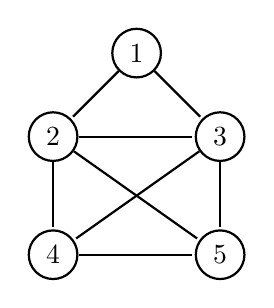
\begin{tikzpicture}[-,>=stealth,shorten >=1pt,auto,node distance=1.5cm, thick,main node/.style={scale=0.9,circle,draw,font=\sffamily\normalsize}]

                \node[circle, draw]  (1) []{1};
                \node[circle, draw]  (2) [below left of = 1]{2};
                \node[circle, draw]  (3) [below right of = 1]{3};
                \node[circle, draw]  (4) [below of = 2]{4};
                \node[circle, draw]  (5) [below of = 3]{5};

                \draw[-] (1) to (2);
                \draw[-] (1) to (3);
                \draw[-] (2) to (3);
                \draw[-] (2) to (4);
                \draw[-] (2) to (5);
                \draw[-] (3) to (4);
                \draw[-] (3) to (5);
                \draw[-] (4) to (5);

                ;
            \end{tikzpicture}

            &\qquad\qquad&

            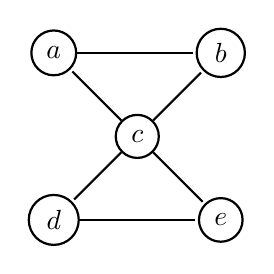
\begin{tikzpicture}[-,>=stealth,shorten >=1pt,auto,node distance=1.5cm, thick,main node/.style={scale=0.9,circle,draw,font=\sffamily\normalsize}]

                \node[circle, draw]  (1) []{$c$};
                \node[circle, draw]  (2) [above left of = 1]{$a$};
                \node[circle, draw]  (3) [above right of = 1]{$b$};
                \node[circle, draw]  (4) [below left of = 1]{$d$};
                \node[circle, draw]  (5) [below right of = 1]{$e$};

                \draw[-] (1) to (2);
                \draw[-] (1) to (3);
                \draw[-] (2) to (3);
                \draw[-] (1) to (4);
                \draw[-] (1) to (5);
                \draw[-] (4) to (5);

                ;
            \end{tikzpicture}
        \end{tabular}
        % \caption{On the left: a simple graph. On the right: a simple digraph.}
    \end{figure}

    Write at least two sentences distinguishing the two structures. Discuss the EF-game played on these structures: for what $k$ can the Duplicator win the $k$-rounds game? For what $k$ can the Spoiler win?

    \begin{proof}[Solution]
        Some properties that can distinguish these two structures are the following:

        \begin{enumerate}
            \item \curlyquotes{$\mathcal G$ contains a vertex of degree 3}, which is represented by the following sentence of rank 5 \centeredeq{0.9}{$\displaystyle \exists x_1 \exists x_2 \exists x_3 \exists x_4 \quad \rbk{\bigwedge_{\substack{1 \le i, j \le 4 \\ i \neq j}}{\lnot(x_i = x_j)}} \land \rbk{\bigwedge_{2 \le i \le 4}{E(x_1, x_i)}} \land \rbk{\forall y \quad \lnot E(x_1, y) \lor \bigvee_{2 \le j \le 4}{(y = x_j)}}$}
            \item \curlyquotes{$\mathcal G$ contains edges as $\mathcal G_1$}, which is represented by the following sentence of rank 5
                \begin{equation*}
                    \begin{split}
                        \exists x_1 \exists x_2 \exists x_3 \exists x_4 \exists x_5 \quad &E(x_1, x_2) \land E(x_1, x_3) \land \\
                                                                                          &E(x_2, x_3) \land E(x_2, x_4) \land E(x_2, x_5) \land \\
                                                                                          &E(x_3, x_4) \land E(x_4, x_5) \land \\
                                                                                          &E(x_4, x_5)
                    \end{split}
                \end{equation*}
                we observe that the edges of $\mathcal G_2$ are not sufficient to distinguish the two sentences, because $\mathcal G_2$ is a subgraph of $\mathcal G_1$
            \item \curlyquotes{$\mathcal G$ contains a cycle of length 5}, which is represented by $C_5$ of the previous exercise, and has rank 5
            \item \curlyquotes{$\mathcal G$ contains a cycle of length 4}, which is represented by $C_4$ of the previous exercise, and has rank 4
            \item \curlyquotes{$\mathcal G$ contains $K_4$ as subgraph}, which is represented by the following sentence having rank 4 $$\exists x_1 \exists x_2 \exists x_3 \exists x_4 \quad \rbk{\bigwedge_{\substack{1 \le i, j \le 4 \\ i \neq j}}{\lnot (x_i = x_j)}} \land \rbk{\bigwedge_{\substack{1 \le i, j \le 4 \\ i \neq j}}{E(x_i, x_j)}}$$
        \end{enumerate}

        These sentences \tit{may seem} to suggest that the two structures are 3-equivalent, meaning that there is no sentence of rank 3 that can distinguish $\mathcal G_1$ from $\mathcal G_2$. For now, let's focus on proving that they are \tit{at least} 2-equivalent.

        \claim{
            The Duplicator wins $G_2(\mathcal G_1, \mathcal G_2)$.
        }{
            Let $s_i$ and $d_i$ be the $i$-th nodes chosen by the Spoiler and the Duplicator, respectively. Then, we can define the following strategy for the Duplicator:

            \begin{itemize}
                \item if $s_1 \in \{1, 4, 5\}$, then the Duplicator chooses $d_1 \in \{a, b, d, e\}$, otherwise if $s_1 \in \{2, 3\}$ then $d_1 = c$
                \item similarly, if $s_1 \in \{a, b, d, e\}$, then the Duplicator chooses $d_1 \in \{1, 4, 5\}$, otherwise if $s_1 = c$ then $d_1 \in \{2, 3\}$
            \end{itemize}

            Then, no matter the choice of $s_2$, the Duplicator can always answer with a node $d_2$ that preserves the partial isomorphism, in fact:

            \begin{itemize}
                \item if $s_2 \sim s_1$, it is guaranteed that there is a vertex $d_2$ in the other structure such that $d_2 \sim d_1$ because $\delta(\mathcal G_1) = \delta(\mathcal G_2) = 2$ --- and the same argument applies if $s_2 \sim d_1$ for finding a vertex $d_2 \sim s_1$
                \item if $s_2 \nsim s_1$, the strategy that we provided for the Duplicator guarantees that there exists at least one vertex $d_2$ in the other structure such that $d_2 \nsim d_1$ --- and the same argument applies if $s_2 \nsim d_1$ for finding a vertex $d_2 \nsim s_1$
            \end{itemize}

            Thus, the Duplicator has a strategy to always win at least 2 rounds, therefore the Duplicator wins $G_2(\mathcal G_1, \mathcal G_2)$ by Ehrenfeucht's theorem.
        }

        Now that we proved that $\mathcal G_1 \equiv_2 \mathcal G_2$, is it true that they are also 3-equivalent? Unfortunately, the following claim proves that this is indeed false.

        \claim{
            The Spoiler wins $G_3(\mathcal G_1, \mathcal G_2)$.
        }{
            The following is a strategy that guarantees the Spoiler to win in 3 rounds:

            \begin{itemize}
                \item let $s_1 \in \{4, 5\}$
                \item by the previous claim, we know that the strategy for the Duplicator to win at least 2 rounds is to choose $d_1 \in \{a, b, d, e\}$, thus we may assume that $d_1 \neq c$
                \item now, let $s_2 = 1$
                \item to preserve the partial isomorphism, we observe that
                    \begin{itemize}
                        \item if $d_1 \in \{a, b\}$, then $d_2 \in \{d, e\}$
                        \item if $d_1 \in \{d, e\}$, then $d_2 \in \{a, b\}$
                    \end{itemize}
                \item now, it suffices for the Spoiler to choose $s_3$ in $\mathcal G_2$ such that $s_3 \sim d_2$ and $s_3 \neq c$: by construction of $\mathcal G_2$, we see that $s_3 \nsim d_1$, but all the vertices in $\{2, 3, 5\}$ are adjacent to $s_1$, which would violate the partial isomorphism
            \end{itemize}
        }

        In fact, we can actually find a property that distinguishes $\mathcal G_1$ from $\mathcal G_2$ which can be written through a sentence of rank 3: \curlyquotes{there are two vertices $x_1$ and $x_2$ of $\mathcal G$ such that for each third vertex $x_3$ there is a $K_3$ as subgraph of $\mathcal G$ such that $V(K_3) = \{x_1, x_2, x_3\}$} $$\exists x_1 \exists x_2 \forall x_3 \quad \rbk{\bigwedge_{\substack{1 \le i, j \le 3 \\ i \neq j}}{\lnot (x_i = x_j)}} \land E(x_1, x_2) \land E(x_2, x_3) \land E(x_3, x_1)$$ Let $x_1$, $x_2$ and $x_3$ be the three choosen vertices --- and we may assume that $x_1 \sim x_2$ otherwise the sentence is trivially unsatisfied. Then, we observe that

        \begin{itemize}
            \item in $\mathcal G_1$ if $\{x_1, x_2\} = \{2, 3\}$, then for any other vertex $x_3 \in \{1, 4, 5\}$ we can always find a $K_3$ having $x_1$, $x_2$ and $x_3$ as its vertices
            \item in $\mathcal G_2$ we have two cases
                \begin{itemize}
                    \item if $\{x_1, x_2\} \subseteq \{a, b, c\}$, the property is unsatisfied for $x_3 \in \{d, e\}$
                    \item if $\{x_1, x_2\} \subseteq \{c, d, e\}$, the property is unsatisfied for $x_3 \in \{a, b\}$
                \end{itemize}
        \end{itemize}

        In conclusion, we have that $\mathcal G_1 \equiv_2 \mathcal G_2$, and that $\mathcal G_1 \not\equiv_3 \mathcal G_2$.
    \end{proof}

    \section{Homework 2}

    \newpage

    \tbf{Exercise 1.1} Let $(W, R)$ be a \tit{quasi-order}; that is, assume that $R$ is transitive and reflexive. Define the binary relation $\sim$ on $W$ by putting $s \sim t \iff R(s, t) \land R(t, s)$.

    \begin{enumerate}[label=(\alph*)]
        \item Show that $\sim$ is an equivalence relation.
    \end{enumerate}

    Let $[s]$ denote the equivalence class of $s$ under this relation, and define the following relation on the collection of equivalence classes: $[s] \le [t] \iff R(s, t)$.

    \begin{enumerate}[label=(\alph*)]
        \setcounter{enumi}{1}
        \item Show that this relation is well-defined.
        \item Show that $\le$ is a partial order.
    \end{enumerate}

    \solution{
        We prove the statements as follows.

        \begin{enumerate}[label=(\alph*)]
            \item To prove that $\sim$ is an equivalence relation, it suffices to show that $\sim$ has the following properties:
                \begin{itemize}
                    \item \tit{reflexivity}: $\forall s \in W \quad R(s, s)$ by reflexivity of $R$, therefore $s \sim s$
                    \item \tit{symmetry}: $\forall s, t \in W \quad s \sim t \iff R(s, t) \land R(t, s) \iff t \sim s$
                    \item \tit{transitivity}: $\forall s, t, u \in W \quad \soe{l}{s \sim t \iff R(s, t) \land R(t, s) \\ t \sim u \iff R(t, u) \land R(u, t)}$ and by transitivity of $R$ we have that
                        \begin{itemize}
                            \item $R(s, t) \land R(t, u) \implies R(s, u)$
                            \item $R(u, t) \land R(t, s) \implies R(u, s)$
                        \end{itemize}

                        and by definition $R(s, u) \land R(u, s) \iff s \sim u$
                \end{itemize}

            \item To prove that $\le$ is well-defined, we need to show that $$\forall s, t, s', t' \quad s \sim s' \land t \sim t' \implies ([s] \le [t] \iff [s'] \le [t'])$$ We observe that

                \begin{itemize}
                    \item $s \sim s' \iff R(s, s') \land R(s', s)$
                    \item $t \sim t' \iff R(t, t') \land R(t', t)$
                \end{itemize}

                therefore, we have that
                
                \begin{itemize}
                    \item $[s] \le [t] \iff R(s, t)$, and by transitivity of $R$ it holds that $R(s', s) \land R(s, t) \implies R(s', t)$; therefore, by transitivity of $R$ again we have that $R(s', t) \land R(t, t') \implies R(s', t') \iff [s'] \le [t']$
                    \item $[s'] \le [t'] \iff R(s', t')$, and by transitivity of $R$ it holds that $R(s', t') \land R(t', t) \implies R(s', t)$; therefore, by transitivity of $R$ again we have that $R(s, s') \land R(s', t) \implies R(s, t) \iff [s] \le [t]$
                \end{itemize}
            \item To prove that $\le$ is a partial order, it suffices to show that $\le$ has the following properties:

                \begin{itemize}
                    \item \tit{reflexivity}: $\forall s \in W \quad R(s, s)$ by reflexivity of $R$, and $R(s, s) \iff [s] \le [s]$
                    \item \tit{antisymmetry}: $\forall s, t \in W \quad \soe{l}{[s] \le [t] \iff R(s, t) \\ \left[t\right] \le [s] \iff R(t, s)} \implies R(s, t) \land R(t, s) \iff s \sim t \iff [s] = [t]$
                    \item \tit{transitivity}: $\forall s, t, u \in W \quad \soe{l}{[s] \le [t] \iff R(s, t) \\  \left[t\right] \le [u] \iff R(t, u)} \implies R(s, t) \land R(t, u)\implies R(s, u)$ by transitivity of $R$, and $R(s, u) \iff [s] \le [u]$
                \end{itemize}
        \end{enumerate}
    }

    \tbf{Exercise 2.2} Let $\mathcal N = (\N, S_1, S_2)$ and $\mathcal B = (\mathbb B, R_1, R_2)$ be the following frames for a modal similarity type with two diamonds $\lozenge_1$, $\lozenge_2$. Here, $\N$ is the set of natural numbers and $\mathbb B$ is the set of strings of 0's and 1's, and the relations are defined by
        \begin{equation*}
            \begin{split}
                S_1(m, n) &\iff n = m + 1 \\
                S_2(m, n) &\iff m > n \\
                R_1(s, t) &\iff t = s0 \lor t = s1 \\
                R_2(s, t) &\iff t \sqsubset s
            \end{split}
        \end{equation*}
        where $t \sqsubset s$ if and only if $t$ is a \tit{proper prefix} of $s$ --- i.e. $t$ is a prefix of $s$ such that $t \neq s$ (thus $t$ can be $\varepsilon$). Which of the following formulas are valid on $\mathcal N$ and $\mathcal B$, respectively?

    \begin{enumerate}[label=(\alph*)]
        \item $(\lozenge_1 p \land \lozenge_2 q) \rightarrow \lozenge_1 (p \land q)$
        \item $(\lozenge_2 p \land \lozenge_2 q) \rightarrow \lozenge_2 (p \land q)$
        \item $(\lozenge_1 p \land \lozenge_1 q \land \lozenge_1 r) \rightarrow (\lozenge_1 (p \land q) \lor \lozenge_1(p \land r) \lor \lozenge_1 (q \land r))$
        \item $p \rightarrow \lozenge_1 \Box_1 p$
        \item $p \rightarrow \lozenge_2 \Box_1 p$
        \item $p \rightarrow \Box_1 \lozenge_2 p$
        \item $p \rightarrow \Box_2 \lozenge_1 p$
    \end{enumerate}

    \solution{
        First, consider the following extension to the $\land$ operator on the inductive definition of satisfiability of formulas.

        \claim{
            Given a model $\mathfrak M = (W, R, V)$, and a state $w \in W$, it holds that $\mathfrak M, w \models \phi \land \psi \iff \mathfrak M , w \models \phi \land \mathfrak M, w \models \psi$.
        }{
            By using De Morgan's law, we have that
            \begin{equation*}
                \begin{split}
                    \mathfrak M, w \models \phi \land \psi = \lnot (\lnot \phi \lor \lnot \psi) &\iff \lnot \mathfrak M, w \models \lnot \phi \lor \lnot \psi \\
                                                                                                &\iff \lnot (\mathfrak M , w \models \lnot \phi \lor \mathfrak M, w \models \lnot \psi) \\
                                                                                                &\iff \lnot (\lnot \mathfrak M, w \models \phi \lor \lnot \mathfrak M, w \models \psi) \\
                                                                                                &\iff \mathfrak M, w \models \phi \land \mathfrak M, w \models \psi
                \end{split}
            \end{equation*}
        }

        For all the following propositions, we will assume that $\mathfrak M = (\N, S_1, S_2, V)$ and $\mathfrak M' = (\mathbb B, R_1, R_2, V)$ are two models over $\mathcal N$ and $\mathcal B$ respectively.
 
        \begin{enumerate}[label=(\alph*)]
            \item $(\lozenge_1 p \land \lozenge_1 q) \rightarrow \lozenge_1 (p \land q)$

                \begin{itemize}
                    \item By the claim, for any $m \in \N$ it holds that
                        \begin{equation*}
                            \begin{split}
                                \mathfrak M, m \models \lozenge_1 p \land \lozenge_1 q &\iff \mathfrak M, m \models \lozenge_1 p \land \mathfrak M, m \models \lozenge_1 q \\
                                                                                       &\iff \soe{l}{\exists n_p \in \N \quad S_1(m, n_p) \land \mathfrak M, n_p \models p \\ \exists n_q \in \N \quad S_1(m, n_q) \land \mathfrak M, n_q \models q} \\
                                                                                       &\iff \soe{l}{\exists n_p \in \N \quad n_p = m + 1 \land n_p \in V(p) \\ \exists n_q \in \N \quad n_q = m + 1 \land n_q \in V(p)} \\
                                                                                       &\iff m + 1 \in V(p) \land m + 1 \in V(q) \\
                                                                                       &\iff m + 1 \in V(p) \cap V(q)
                            \end{split}
                        \end{equation*}
                        and again, by the claim we have that
                        \begin{equation*}
                            \begin{split}
                                \mathfrak M, m \models \lozenge_1 ( p \land q) &\iff \exists n \in \N \quad S_1 (m , n) \land \mathfrak M, n \models p \land q \\
                                                                               &\iff \exists n \in \N \quad n = m + 1 \land (\mathfrak M, n \models p \land \mathfrak M, n \models q) \\
                                                                               &\iff \exists n \in \N \quad n = m + 1 \land (n \in V(p) \land n \in V(q)) \\
                                                                               &\iff \exists n \in \N \quad n = m + 1 \land n \in V(p) \cap V(q) \\
                                                                               &\iff m + 1 \in V(p) \cap V(q)
                            \end{split}
                        \end{equation*}
                        from which we conclude that $$\mathfrak M, m \models \lozenge_1 p \land \lozenge_1 q \iff m + 1 \in V(p) \cap V(q) \iff \mathfrak M, m \models \lozenge_1(p \land q)$$ implying that the formula is valid on $\mathcal N$.
                    \item By the claim, for any $s \in \mathbb B$ it holds that
                        \begin{equation*}
                            \begin{split}
                                \mathfrak M', s \models \lozenge_1 p \land \lozenge_1 q &\iff \mathfrak M', s \models \lozenge_1 p \land \mathfrak M', s \models \lozenge_1 q \\
                                                                                        &\iff \soe{l}{\exists t_p \in \mathbb B \quad R_1(s, t_p) \land \mathfrak M', t_p \models p \\ \exists t_q \in \mathbb B \quad R_1(s, t_q) \land \mathfrak M', t_q \models q} \\
                                                                                        &\iff \soe{l}{\exists t_p \in \mathbb B \quad (t_p = s0 \lor t_p = s1) \land t_p \in V(p) \\ \exists t_q \in \mathbb B \quad (t_q = s0 \lor t_q = s1) \land t_q \in V(q)} \\
                                                                                        &\iff \soe{l}{s0 \in V(p) \lor s1 \in V(p) \\ s0 \in V(q) \lor s1 \in V(q)} \\
                                                                                        &\iff \{s0, s1\} \cap V(p) \neq \varnothing \land \{s0, s1\} \cap V(q) \neq \varnothing
                            \end{split}
                        \end{equation*}
                        and again, by the claim we have that
                        \begin{equation*}
                            \begin{split}
                                \mathfrak M', s \models \lozenge_1(p \land q) \models &\iff \exists t \in \mathbb B \quad R_1(s, t) \land \mathfrak M', t \models p \land q \\
                                                                                      &\iff \exists t \in \mathbb B \quad (t = s0 \lor t = s1) \land (\mathfrak M', t \models p \land \mathfrak M', t \models q) \\
                                                                                      &\iff \exists t \in \mathbb B \quad (t = s0 \lor t = s1) \land (t \in V(p) \land t \in V(q)) \\
                                                                                      &\iff \exists t \in \mathbb B \quad (t = s0 \lor t = s1) \land t \in V(p) \cap V(q) \\
                                                                                      &\iff s0 \in V(p) \cap V(q) \lor s1 \in V(p) \cap V(q) \\
                                                                                      &\iff \{s0, s1\} \cap V(p) \cap V(q) \neq \varnothing
                            \end{split}
                        \end{equation*}
                        Now suppose $V(p) = \{s0\}$ and $V(q) = \{s1\}$; then we have that $\{s0, s1\} \cap V(p) = \{s0\} \neq \varnothing \land \{s0, s1\} \cap V(q) = \{s1\} \neq \varnothing \iff \mathfrak M', s \models \lozenge_1 p \land \lozenge_1 q$ although $\{s0, s1\} \cap V(p) \cap V(q) = \{s0, s1\} \cap \varnothing = \varnothing \iff \mathfrak M', s \not\models \lozenge_1(p \land q)$, implying that the formula is not valid on $\mathcal B$.
                \end{itemize}
            \item $(\lozenge_2 p \land \lozenge_2 q) \rightarrow \lozenge_2 (p \land q)$
                \begin{itemize}
                    \item By definition, for any $m \in \N$ it holds that
                        \begin{equation*}
                            \begin{split}
                                \mathfrak M, m \models \lozenge_2 p \land \lozenge_2 q &\iff \mathfrak M, m \models \lozenge_2 p \land \mathfrak M, m \models \lozenge_2 q \\
                                                                                       &\iff \soe{l}{\exists n_p \in \N \quad S_2(m, n_p) \land \mathfrak M, n_p \models p \\ \exists n_q \in \N \quad S_2(m, n_q) \land \mathfrak M, n_q \models q} \\
                                                                                       &\iff \soe{l}{\exists n_p \in \N \quad m > n_p \land n_p \in V(p) \\ \exists n_q \in \N \quad m > n_q \land n_q \in V(q)}
                            \end{split}
                        \end{equation*}
                        and again, by the claim we have that
                        \begin{equation*}
                            \begin{split}
                                \mathfrak M, m \models \lozenge_2 (p \land q) &\iff \exists n \in \N \quad S_2(m, n) \land \mathfrak M, n \models p \land q \\
                                                                             &\iff \exists n \in \N \quad m > n \land (\mathfrak M, n \models P \land \mathfrak M , n \models q) \\
                                                                             &\iff \exists n \in \N \quad m > n \land (n \in V(p) \land n \in V(q)) \\
                                                                             &\iff \exists n \in \N \quad m > n \land n \in V(p) \cap n \in V(q)
                            \end{split}
                        \end{equation*}
                        Now take an $n \ge 2$, and consider $n_p, n_q \in \N$ such that $n_p \neq n_q \land n > n_p, n_q$, and suppose that $V(p) = \{n_p\}$ and $V(q) = \{n_q\}$; then we have that $\soe{l}{\exists n_p \in \N \quad n > n_p \land n_p \in V(p) \\ \exists n_q \in \N \quad n > n_q \land n_q \in V(q)} \iff \mathfrak M, m \models \lozenge_2 p \land \lozenge_2 q$ although $n_p \neq n_q \implies V(p) \cap V(q) = \varnothing \implies \nexists n \in \N \quad m > n \land n \in V(p) \cap V(q) \iff \mathfrak M, m \not\models \lozenge_2(p \land q)$, implying that the formula is not valid on $\mathcal N$.
                    \item By the claim, for any $s \in \mathbb B$ it holds that
                        \begin{equation*}
                            \begin{split}
                                \mathfrak M', s \models \lozenge_2 p \land \lozenge_2 q &\iff \mathfrak M', s \models \lozenge_2 p \land \mathfrak M', s \models \lozenge_2 q \\
                                                                                        &\iff \soe{l}{\exists t_p \in \mathbb B \quad R_2(s, t_p) \land \mathfrak M', t_p \models p \\ \exists t_q \in \mathbb B \quad R_2(s, t_q) \land \mathfrak M', t_q \models q} \\
                                                                                        &\iff \soe{l}{\exists t_p \in \mathbb B \quad t_p \sqsubset s \land t_p \in V(p) \\ \exists t_q \in \mathbb B \quad t_q \sqsubset s \land t_q \in V(p)}
                            \end{split}
                        \end{equation*}
                        and again, by the claim we have that
                        \begin{equation*}
                            \begin{split}
                                \mathfrak M's \models \lozenge_2(p \land q) &\iff \exists t \in \mathbb B \quad t \sqsubset s \land (\mathfrak M', t \models p \land \mathfrak M', t \models q) \\
                                                                            &\iff \exists t \in \mathbb B \quad t \sqsubset s \land (t \in V(p) \land t \in V(q)) \\
                                                                            &\iff \exists t \in \mathbb B \quad t \sqsubset s \land t \in V(p) \cap V(q)
                            \end{split}
                        \end{equation*}
                        Now take $s = 000$, consider $t_p = 0$ and $t_q = 0$, and suppose that $V(p) = \{t_p\} = \{0\}$ and $V(q) = \{t_q\} = \{00\}$; we observe that $t_p = 0 \sqsubset 000 = s$ and $t_q = 00 \sqsubset 000 = s$, therefore $\soe{l}{\exists t_p \in \mathbb B \quad t_p \sqsubset s \land t_p \in V(p) \\ \exists t_q \in \mathbb B \quad t_q \sqsubset s \land t_q \in V(q)} \iff \mathfrak M', s \models \lozenge_2 p \land \lozenge_2 q$ although $V(p) \cap V(q) = \{t_p\} \cap \{t_q\} = \{0\} \cap \{00\} = \varnothing \implies \nexists t \in \mathbb B \quad t \sqsubset s \land t \in V(p) \cap V(q) \iff \mathfrak M', s \not\models \lozenge_2 (p \land q)$, implying that the formula is not valid on $\mathcal B$.
                \end{itemize}
            \item $(\lozenge_1 p \land \lozenge_1 q \land \lozenge_1 r) \rightarrow (\lozenge_1 (p \land q) \lor \lozenge_1 (p \land r) \lor \lozenge_1 (q \land r))$
                \begin{itemize}
                    \item By the claim, for any $m \in \N$ it holds that
                        \begin{equation*}
                            \begin{split}
                                \mathfrak M, m \models \lozenge_1 p \land \lozenge_1 q \land \lozenge_1 r &\iff \mathfrak M, m \models \lozenge_1 p \land \mathfrak M, m \models \lozenge_1 q \land \mathfrak M, m \models \lozenge_1 r \\
                                                                                                          &\iff \soe{l}{\exists n_p \in \N \quad S_1(m, n_p) \land \mathfrak M, n_p \models \lozenge_1 p \\ \exists n_q \in \N \quad S_1(m, n_q) \land \mathfrak M, n_q \models \lozenge_1 q \\ \exists n_r \in \N \quad S_1(m, n_r) \land \mathfrak M, n_r \models \lozenge_1 r} \\
                                                                                                          &\iff \soe{l}{\exists n_p \in \N \quad n_p = m + 1 \land n_p \in V(p) \\ \exists n_q \in \N \quad n_q = m + 1 \land n_q \in V(q) \\ \exists n_r \in \N \quad n_r = m + 1 \land n_r \in V(r)} \\
                                                                                                          &\iff \soe{l}{m + 1 \in V(p) \\ m + 1 \in V(q) \\ m + 1 \in V(r)} \\
                                                                                                          &\iff m + 1 \in V(p) \cap V(q) \cap V(r)
                            \end{split}
                        \end{equation*}
                        and again, by the claim we have that
                        % \begin{equation*}
                        \centeredeq{1}{$
                            \begin{alignedat}{2}
                                \mathfrak M , m \models \lozenge_1 (p \land q) \lor \lozenge_1 (p \land r) \lor \lozenge_1 (q \land r) &\iff &&(\mathfrak M, m \models \lozenge_1 (p \land q)) \\
                                                                                                                                       &     &&\lor (\mathfrak M, m \models \lozenge_1 (p \land r)) \\
                                                                                                                                       &     &&\lor (\mathfrak M, m \models \lozenge_1 (q \land r)) \\
                                                                                                                                       &\iff &&(\exists n_1 \in \N \quad S_1(m, n_1) \land \mathfrak M, n_1 \models p \land q) \\
                                                                                                                                       &     &&\lor (\exists n_2 \in \N \quad S_1(m, n_2) \land \mathfrak M, n_2 \models p \land r) \\
                                                                                                                                       &     &&\lor (\exists n_3 \in \N \quad S_1(m, n_3) \land \mathfrak M, n_3 \models q \land r) \\
                                                                                                                                       &\iff &&(\exists n_1 \in \N \quad n_1 = m + 1 \land n_1 \in V(p) \cap V(q)) \\
                                                                                                                                       &     &&\lor (\exists n_2 \in \N \quad n_2 = m + 1 \land n_2 \in V(p) \cap V(r)) \\
                                                                                                                                       &     &&\lor (\exists n_3 \in \N \quad n_3 = m + 1 \land n_3 \in V(q) \cap V(r)) \\
                                                                                                                                       &\iff &&(m + 1 \in V(p) \cap V(q)) \\
                                                                                                                                       &     &&\lor (m + 1 \in V(p) \cap V(r)) \\
                                                                                                                                       &     &&\lor (m + 1 \in V(q) \cap V(r))
                            \end{alignedat}
                        $}
                        % \end{equation*}
                        Hence, we see that
                        \begin{equation*}
                            \begin{split}
                                \mathfrak M, m \models \lozenge_1 p \land \lozenge_1 q \land \lozenge_1 r &\iff m + 1 \in V(p) \cap V(q) \cap V(r) \\
                                                                                                          &\implies \soe{l}{m + 1 \in V(p) \cap V(q) \\ m + 1 \in V(p) \cap V(r) \\ m + 1 \in V(q) \cap V(r)} \\
                                                                                                          &\iff \mathfrak M, m \models \lozenge_1(p \land q) \lor \lozenge_1 (p \land r) \lor \lozenge_1 (q \land r)
                            \end{split}
                        \end{equation*}
                        implying that the formula is valid in $\mathcal N$.
                    \item By the claim, for any $s \in \mathbb B$ it holds that
                        \begin{equation*}
                            \begin{split}
                                \mathfrak M', s \models \lozenge_1 p \land \lozenge_1 q \land \lozenge_1 r &\iff \mathfrak M', s \models \lozenge_1 p \land \mathfrak M', s \models \lozenge_1 q \land \mathfrak M', s \models \lozenge_1 r \\
                                                                                                           &\iff \soe{l}{\exists t_p \in \mathbb B \quad R_1(s, t_p) \land \mathfrak M', t_p \models p \\ \exists t_q \in \mathbb B \quad R_1(s, t_q) \land \mathfrak M', t_q \models q \\ \exists t_r \in \mathbb B \quad R_1(s, t_r) \land \mathfrak M', t_r \models r} \\
                                                                                                           &\iff \soe{l}{\exists t_p \in \mathbb B \quad (t_p = s0 \lor t_p = s1) \land t_p \in V(p) \\ \exists t_p \in \mathbb B \quad (t_q = s0 \lor t_q = s1) \land t_q \in V(q) \\ \exists t_r \in \mathbb B \quad (t_r = s0 \lor t_r = s1) \land t_r \in V(r)} \\
                                                                                                           &\iff \soe{l}{\{s0, s1\} \cap V(p) \neq \varnothing \\ \{s0, s1\} \cap V(q) \neq \varnothing \\ \{s0, s1\} \cap V(r) \neq \varnothing}
                            \end{split}
                        \end{equation*}
                        and again, by the claim we have that
                        \centeredeq{1}{$
                            \begin{alignedat}{2}
                                \mathfrak M', s \models \lozenge_1 (p \land q) \lor \lozenge_1 (p \land r) \lor \lozenge_1 (q \land r) &\iff &&(\mathfrak M', s \models \lozenge_1(p \land q)) \\
                                                                                                                                       &     &&\lor (\mathfrak M', s \models \lozenge_1 (p \land r)) \\
                                                                                                                                       &     &&\lor (\mathfrak M', s \models \lozenge_1 (q \land r)) \\
                                                                                                                                       &\iff &&(\exists t_1 \in \mathbb B \quad R_1(s, t_1) \land \mathfrak M', t_1 \models p \land q) \\
                                                                                                                                       &     &&\lor (\exists t_2 \in \mathbb B \quad R_1(s, t_2) \land \mathfrak M', t_2 \models p \land r) \\
                                                                                                                                       &     &&\lor (\exists t_3 \in \mathbb B \quad R_1(s, t_3) \land \mathfrak M', t_3 \models q \land r) \\
                                                                                                                                       &\iff &&(\exists t_1 \in \mathbb B \quad (t_1 = s0 \lor t_1 = s1) \land t_1 \in V(p) \cap V(q)) \\
                                                                                                                                       &     &&\lor (\exists t_2 \in \mathbb B \quad (t_2 = s0 \lor t_2 = s1) \land t_2 \in V(p) \cap V(r)) \\
                                                                                                                                       &     &&\lor (\exists t_3 \in \mathbb B \quad (t_3 = s0 \lor t_3 = s1) \land t_3 \in V(q) \cap V(r)) \\
                                                                                                                                       &\iff &&\{s0, s1\} \cap V(p) \cap V(q) \neq \varnothing \\
                                                                                                                                       &     &&\lor \{s0, s1\} \cap V(p) \cap V(q) \neq \varnothing \\
                                                                                                                                       &     &&\lor \{s0, s1\} \cap V(q) \cap V(r) \neq \varnothing
                            \end{alignedat}
                        $}
                        Now suppose that $\mathfrak M', s \models \lozenge_1 p \land \lozenge_1 q \land \lozenge_1 r$, which happens if and only if $\soe{l}{\{s0, s1\} \cap V(p) \neq \varnothing \\ \{s0, s1\} \cap V(q) \neq \varnothing \\ \{s0, s1\} \cap V(r) \neq \varnothing}$ as proved previously; by the pigeonhole principle, since there are 2 strings in $\{s0, s1\}$ and we have 3 sets $V(p)$, $V(q)$ and $V(r)$, there must be at least one string $x \in \{s0, s1\}$ such that $x \in V(a) \cap V(b)$, where $a, b \in \{p, q, r\}$ distinct. Without loss of generality, suppose that $x = s0$ and $a = p$ and $b = q$; then we have that
                        \begin{equation*}
                            \begin{split}
                                x = s0 \in V(p) \cap V(q) &\implies x \in \{s0, s1\} \cap V(p) \cap V(q) \\
                                                          &\implies \{s0, s1\} \cap V(p) \cap V(q) \neq \varnothing \\
                                                          &\implies \mathfrak M', s \models \lozenge_1 (p \land q) \lor \lozenge_1 (p \land r) \lor \lozenge_1(q \land r)
                            \end{split}
                        \end{equation*}
                        implying that the formula is valid on $\mathcal B$.
                \end{itemize}
            \item $p \rightarrow \lozenge_1 \Box_2 p$
                \begin{itemize}
                    \item By definition, for any $m \in \N$ it holds that
                        \begin{equation*}
                            \begin{split}
                                \mathfrak M, m \models \lozenge_1 \Box_2 p &\iff \exists n \in \N \quad S_1(m, n) \land \mathfrak M, n \models \Box_2 p \\
                                                                           &\iff \exists n \in \N \quad n = m + 1 \land (\forall k \in \N \quad S_2(n, k) \implies \mathfrak M, k \models p) \\
                                                                           &\iff \exists n \in \N \quad n = m + 1 \land (\forall k \in \N \quad n > k \implies k \in V(p)) \\
                                                                           &\iff \forall k \in \N \quad m + 1 > k \implies k \in V(p) \\
                                                                           &\iff V(p) = \{k \in \N \mid m + 1 > k\}
                            \end{split}
                        \end{equation*}
                        Now take $m = 1 \in \N$, and suppose $V(p) = \{m\} = \{1\}$; then $m \in V(p) \iff \mathfrak M, m \models p$, however for instance $k = 0 \in \N$ is such that $m + 1 = 1 + 1 = 2 > 0 = k$ although $k = 0 \notin V(p)$, therefore $\exists k \in \N \quad m + 1 > k \land k \notin V(p) \implies V(p) \neq \{k \in \N \mid m + 1 > k\} \iff \mathfrak M, m \not\models \lozenge_1 \Box_2 p$ which implies that the formula is not valid on $\mathcal N$.
                    \item By definition, for any $s \in \mathbb B$ it holds that
                        \begin{equation*}
                            \begin{split}
                                \mathfrak M', s \models \lozenge_1 \Box_2 p &\iff \exists t \in \mathbb B \quad R_1(s, t) \land \mathfrak M', t \models \Box_2 p \\
                                                                           &\iff \exists t \in \mathbb B \quad (t = s0 \lor t = s1) \land (\forall u \in \mathbb B \quad R_2(t, u) \implies \mathfrak M', u \models p) \\
                                                                           &\iff \exists t \in \mathbb B \quad (t = s0 \lor t = s1) \land (\forall u \in \mathbb B \quad u \sqsubset t \implies u \in V(p))
                            \end{split}
                        \end{equation*}
                        Now take $s = 00 \in \mathbb B$, and suppose $V(p) = \{s\} = \{00\}$; then $s \in V(p) \iff \mathfrak M', s \models p$, however if $t = s0$ or $t = s1$, there still is $u = 0$ such that $u = 0\sqsubset 00 = t$ although $u = 0 \notin V(p)$, therefore $(t = s0 \lor t = s1) \implies (\exists u \in \mathbb B \quad u \sqsubset t \land u \notin V(p)) \iff \mathfrak M', s \not\models \lozenge_1 \Box_2 p$ which implies that the formula is not valid on $\mathcal B$.
                \end{itemize}
            \item $p \rightarrow \lozenge_2 \Box_1 p$
                \begin{itemize}
                    \item By definition, for any $m \in \N$ it holds that
                        \begin{equation*}
                            \begin{split}
                                \mathfrak M, m \models \lozenge_2 \Box_1 p &\iff \exists n \in \N \quad S_2(m, n) \land \mathfrak M, n \models \Box_1 p \\
                                                                           &\iff \exists n \in \N \quad m > n \land (\forall k \in \N \quad S_1(n, k) \implies \mathfrak M, k \models p) \\
                                                                           &\iff \exists n \in \N \quad m > n \land (\forall k \in \N \quad k = n + 1 \implies k \in V(p)) \\
                                                                           &\iff \exists n \in \N \quad m > n \land n + 1 \in V(p)
                            \end{split}
                        \end{equation*}
                        Now take $m = 0 \in \N$, and suppose $V(p) = \{m\} = \{0\}$; then $m \in V(p) \iff \mathfrak M, m \models p$, however there is no $n \in \N$ such that $m = 0 > n$, therefore $\nexists n \in \N \quad m > n \land n + 1 \in V(p) \iff \mathfrak M, m \not\models \lozenge_2 \Box_1 p$ which implies that the formula is not valid on $\mathcal N$.
                    \item By definition, for any $s \in \mathbb B$ it holds that
                        \begin{equation*}
                            \begin{split}
                                \mathfrak M', s \models \lozenge_2 \Box_1 p &\iff \exists t \in \mathbb B \quad R_2(s, t) \land \mathfrak M', t \models \Box_1 p \\
                                                                            &\iff \exists t \in \mathbb B \quad t \sqsubset s \land (\forall u \in \mathbb B \quad R_1(t, u) \implies \mathfrak M', u \models p) \\
                                                                            &\iff \exists t \in \mathbb B \quad t \sqsubset s \land (\forall u \in \mathbb B \quad (u = t0 \lor u = t1) \implies u \in V(p)) \\
                                                                            &\iff \exists t \in \mathbb B \quad t \sqsubset s \land (t0 \in V(p) \lor t1 \in V(p))
                            \end{split}
                        \end{equation*}
                        Now take $s = \varepsilon \in \mathbb B$, and suppose $V(p) = \{s\} = \{\varepsilon\}$; then $s \in V(p) \iff \mathfrak M', s \models p$, however there is no $t \in \mathbb B$ such that $t \sqsubset s$, therefore $\nexists t \in \mathbb B \quad t \sqsubset s \land (t0 \in V(p) \lor t1 \in V(p)) \iff \mathfrak M', s \not\models \lozenge_2 \Box_1 p$ which implies that the formula is not valid on $\mathcal B$.
                \end{itemize}
            \item $p \rightarrow \Box_1 \lozenge_2 p$
                \begin{itemize}
                    \item By definition, for any $m \in \N$ it holds that
                        \begin{equation*}
                            \begin{split}
                                \mathfrak M, m \models \Box_1 \lozenge_2 p &\iff \forall n \in \N \quad S_1(m, n) \implies \mathfrak M, n \models \lozenge_2 p \\
                                                                         &\iff \forall n \in \N \quad n = m + 1 \implies (\exists k \in \N \quad S_2(n, k) \land \mathfrak M, k \models p) \\
                                                                         &\iff \forall n \in \N \quad n = m + 1 \implies (\exists k \in \N \quad n > k \land k \in V(p)) \\
                                                                         &\iff \exists k \in \N \quad m + 1 > k \land k \in V(p)
                            \end{split}
                        \end{equation*}
                        Now suppose $m \in V(p) \iff \mathfrak M, m \models p$; we observe that for every $m \in \N$ it holds that $m + 1 > m$, therefore $m + 1 > m \land m \in V(p) \iff \exists k \in \N \quad m + 1 > k \land k \in V(p) \iff \mathfrak M, m \models \Box_1 \lozenge_2 p$, which implies that the formula is valid on $\mathcal N$.
                    \item By definition, for any $s \in \mathbb B$ it holds that
                        \begin{equation*}
                            \begin{split}
                                \mathfrak M', s \models \Box_1 \lozenge_2 p &\iff \forall t \in \mathbb B \quad R_1(s, t) \implies \mathfrak M', t \models \lozenge_2 p \\
                                                                            &\iff \forall t \in \mathbb B \quad (t = s0 \lor t = s1) \implies (\exists u \in \mathbb B \quad R_2(t, u) \land \mathfrak M', u \models p) \\
                                                                            &\iff \forall t \in \mathbb B \quad (t = s0 \lor t = s1) \implies (\exists u \in \mathbb B \quad u \sqsubset t \land u \in V(p))
                            \end{split}
                        \end{equation*}
                        Now suppose $s \in V(p) \iff \mathfrak M', s \models p$; we observe that for every $s \in \mathbb B$ it holds that $s \sqsubset s0, s1$, therefore $\exists u \in \mathbb B \quad (u \sqsubset s0 \lor u \sqsubset s1) \land u \in V(p) \iff \mathfrak M', s \models \Box_1 \lozenge_2 p$, which implies that the formula is valid on $\mathcal B$.
                \end{itemize}
            \item $p \rightarrow \Box_2 \lozenge_1 p$
                \begin{itemize}
                    \item By definition, for any $m \in \N$ it holds that
                        \begin{equation*}
                            \begin{split}
                                \mathfrak M , m \models \Box_2 \lozenge_1 p &\iff \forall n \in \N \quad S_2(m, n) \implies \mathfrak M, n \models \lozenge_2 p \\
                                                                            &\iff \forall n \in \N \quad m > n \implies (\exists k \in \N \quad S_1(n, k) \land \mathfrak M, k \models p) \\
                                                                            &\iff \forall n \in \N \quad m > n \implies (\exists k \in \N \quad k = n + 1 \land k \in V(p)) \\
                                                                            &\iff \forall n \in \N \quad m > n \implies n + 1 \in V(p)
                            \end{split}
                        \end{equation*}
                        Now take $m = 2 \in \N$, and suppose $V(p) = \{m\} = \{2\}$; then $m \in V(p) \iff \mathfrak M, m \models p$, however for instance $n = 0 \in \N$ is such that $m = 2 > 0 = n$ and $n + 1 = 0 + 1 = 1 \notin V(p)$, therefore $\exists n \in \N \quad m > n \land n + 1 \notin V(p) \iff \mathfrak M , m \not\models \Box_2 \lozenge_1 p$, which implies that the formula is not valid on $\mathcal N$.
                    \item By definition, for any $s \in \mathbb B$ it holds that
                        \begin{equation*}
                            \begin{split}
                                \mathfrak M', s \models \Box_2 \lozenge_1 p &\iff \forall t \in \mathbb B \quad R_2(s, t) \implies \mathfrak M', t \models \lozenge_2 p \\
                                                                            &\iff \forall s \in \mathbb B \quad t \sqsubset s \implies (\exists u \in \mathbb B \quad R_1(t, u) \land \mathfrak M', u \models p) \\
                                                                            &\iff \forall s \in \mathbb B \quad t \sqsubset s \implies (\exists u \in \mathbb B \quad (u = t0 \lor u = t1) \implies u \in V(p))
                            \end{split}
                        \end{equation*}
                        Now take $s = 000 \in \mathbb B$, and suppose $V(p) = \{s\} = \{000\}$; then $s \in V(p) \iff \mathfrak M', s \models p$, however for instance $t = 0 \in \mathbb B$ is such that $t = 0 \sqsubset 000 = s$ although there is no $u = t0 = 00$ or $u = t1 = 01$ such that $u \in V(p)$, therefore $\exists t \in \mathbb B \quad t \sqsubset u \land (\nexists u \in \mathbb \quad (u = t0 \lor u = t1) \land u \in V(p)) \iff \mathfrak M', s \not\models \Box_2 \lozenge_1 p$ which implies that the formula is not valid on $\mathcal B$.
                \end{itemize}
        \end{enumerate}
    }

    \tbf{Exercise 3.2} Consider the basic modal language, and the tuple $\mathfrak f = (\N, <, A)$ where $A$ is the collection of finite and co-finite subsets of $\N$. Show that $\mathfrak f$ is a general frame.

    \solution{
        First, consider the follwing two claims.

        \claim[Claim 1]{
            If $X \subseteq \N$ is finite, and $Y \subseteq \N$ is co-finite, then $X \cup Y$ is co-finite.
        }{
            Since $X$ is finite, $\N - X$ is finite, and since $Y$ is co-finite, $\N - Y$ is finite; this implies that $$\N - (X \cup Y) = (\N - X) \cap (\N - Y)$$ is the intersection of a co-finite and a finite set. In particular, we observe that

            \begin{itemize}
                \item such intersection will be a subset of $\N - Y$ by definition of intersection
                \item $\N - Y$ is finite
                \item a subset of a finite set is always finite
            \end{itemize}
            
            concluding that such intersection must be finite as well. Lastly, by definition we have that $\N - (X \cup Y)$ is finite if and only if $X \cup Y$ is co-finite.
        }

        \claim[Claim 2]{
            If $X, Y \subseteq \N$ are co-finite, then $X \cup Y$ is co-finite.
        }{
            By repeating the same argument of the previous claim, we have that $\N - (X \cup Y) = (\N - X) \cap (\N - Y)$ except that in this case both $\N - X$ and $\N - Y$ are finite, which implies that their intersection must be finite, hence $\N - (X \cup Y)$ is co-finite by definition.
        }

        To prove that $\mathfrak f$ is a general frame, it suffices to prove that the set $A$ is closed under the following operations

        \begin{itemize}
            \item \tit{union}: fix two sets $X, Y \in A$; then, by definition of $A$, we have that
                \begin{itemize}
                    \item if both $X$ and $Y$ are finite, then $X \cup Y$ is finite, hence $X \cup Y \in A$
                    \item without loss of generality, if $X$ is finite and $Y$ is co-finite, by Claim 1 $X \cup Y$ is co-finite, therefore $X \cup Y \in A$
                    \item if both $X$ and $Y$ are finite, then $X \cup Y$ is co-finite by Claim 2, therefore $X \cup Y \in A$
                \end{itemize}
            \item \tit{relative complement}: fix a set $X \in A$; then, by definition of $A$ we trivially have that

                \begin{itemize}
                    \item if $X$ is finite, then $\N - X$ is co-finite, hence $\N - X \in A$
                    \item if $X$ is co-finite, then $\N - X$ is finite, hence $\N - X \in A$
                \end{itemize}
            \item \tit{modal operations}: assume that \curlyquotes{<} is the relation referring to a unary modal operator $\abk{<}$, and fix a set $X \in A$; by definition, we have that $$m_{\abk{<}}(X) = \{n \in \N \mid \exists x \in X \quad n < x\}$$ therefore, we have that

                \begin{itemize}
                    \item if $X$ is finite, then $$m_{\abk{<}}(X)= \{n \in \N \mid n < \max(X)\}$$ therefore $m_{\abk{<}}(X)$ is an \curlyquotes{initial segment of $\N$}, implying that it is finite, hence $m_{\abk <}(X) \in A$
                    \item if $X$ is co-finite, then $\N - X$ is finite, implying that $X$ is infinite; this implies that $\max (X)$ is not defined, therefore $$m_{\abk <}(X) = \N \implies \N - m_{\abk <}(X) = \N - \N = \varnothing$$ and since $\varnothing$ is finite, we conclude that $m_{\abk <}(X)$ is co-finite, thus $m_{\abk <}(X) \in A$
                \end{itemize}
        \end{itemize}
    }

    \tbf{Exercise 4.3} Let $\Sigma$ be a set of formulas in the basic modal language, and let $\textsf M$ denote the class of all models. Show that $\Sigma \models_{\textsf M}^g \phi$ if and only if $\{\Box ^n \sigma \mid \sigma \in \Sigma, n \in \N\} \models_{\textsf M} \phi$.

    \solution{
        Let $\Pi := \{\Box ^n \sigma \mid \sigma \in \Sigma, n \in \N\}$. We are going to split the two directions of the proof into two claims.

        \claim{
            If $\Sigma \models_{\textsf M}^g \phi$, then $\Pi \models_{\textsf M} \phi$.
        }{
            Assume that $\Sigma \models_{\textsf M}^g \phi$; fix a model $\mathfrak M$ defined over a domain $W$, and a world $w \in W$. Suppose that $\mathfrak M, w \models \Pi$; then, by the claim of Exercise 2.2 we know that
            \begin{equation*}
                \begin{split}
                         & \forall \sigma \in \Sigma, n \in \N \quad \mathfrak M, w \models \Box^n \sigma \\
                    \iff & \forall \sigma \in \Sigma, n \in \N, x_1, \ldots, x_n \in W \quad w \stackrel{R}{\to} x_1 \stackrel{R}{\to} \ldots \stackrel{R}{\to} x_n \implies \mathfrak M, x_n \models \sigma
                \end{split}
            \end{equation*}
            where $a \stackrel{R}{\to} b \iff R(a, b)$.

            Now, consider the following restriction of $W$ $$W_w := \{v \in W_w \mid \exists n \in \N, x_1, \ldots, x_{n - 1} \in W \quad w \stackrel{R}{\to} x_1 \stackrel{R}{\to} \ldots \stackrel{R}{\to} x_{n - 1} \stackrel{R}{\to} v\}$$ where $v \in W_w$ if and only if $v$ can be $R$-reached from $w$ through a sequence of $R$-accessible elements. Moreover, consider the following restriction of $R$ $$R_w := (W_w \times W_w) \cap R$$ in which we consider the tuples of $R$ that connect elements of $W_w$. Then, consider a model $\mathfrak M_w$ such that $\mathfrak M_w = (W_w, R_w, V_w)$ where $$V_w = W_w \cap V$$

            Consider some $x_1, \ldots, x_n \in W$ such that $w \stackrel{R}{\to} x_1 \stackrel{R}{\to} \ldots \stackrel{R}{\to} x_n$; by definition of $W_w$, this implies that all $x_1, \ldots, x_n$ are $R$-reachable from $w$, which implies that $x_1, \ldots, x_n \in W_w$; this means that
            \begin{equation*}
                \begin{split}
                         & \forall \sigma \in \Sigma, n \in \N, x_1, \ldots, x_n \in W \quad w \stackrel{R}{\to} x_1 \stackrel{R}{\to} \ldots \stackrel{R}{\to} x_n \implies \mathfrak M, x_n \models \sigma \\
                    \implies & \forall \sigma \in \Sigma, n \in \N, x_1 \ldots, x_n \in W_W \quad w \stackrel{R}{\to} x_1 \stackrel{R}{\to} \ldots \stackrel{R}{\to} x_n \implies \mathfrak M, x_n \models \sigma
                \end{split}
            \end{equation*}
            Moreover, since $x_1, \ldots, x_n$ are elements of $W_w$, by definition of $R_w$ it holds that
            \begin{equation*}
                \begin{split}
                    & \forall \sigma \in \Sigma, n \in \N, x_1 \ldots, x_n \in W_W \quad w \stackrel{R}{\to} x_1 \stackrel{R}{\to} \ldots \stackrel{R}{\to} x_n \implies \mathfrak M, x_n \models \sigma \\
                    \implies & \forall \sigma \in \Sigma, n \in \N, x_1 \ldots, x_n \in W_W \quad w \stackrel{R_w}{\to} x_1 \stackrel{R_w}{\to} \ldots \stackrel{R_w}{\to} x_n \implies \mathfrak M, x_n \models \sigma
                \end{split}
            \end{equation*}
            Furthermore, since $W_w \subseteq W$ and $R_w \subseteq R$, by definition of $\mathfrak M_w$ we get that
            \begin{equation*}
                \begin{split}
                    & \forall \sigma \in \Sigma, n \in \N, x_1 \ldots, x_n \in W_W \quad w \stackrel{R_w}{\to} x_1 \stackrel{R_w}{\to} \ldots \stackrel{R_w}{\to} x_n \implies \mathfrak M, x_n \models \sigma \\
                    \implies & \forall \sigma \in \Sigma, n \in \N, x_1 \ldots, x_n \in W_W \quad w \stackrel{R_w}{\to} x_1 \stackrel{R_w}{\to} \ldots \stackrel{R_w}{\to} x_n \implies \mathfrak M_w, x_n \models \sigma
                \end{split}
            \end{equation*}
            This observation concludes that
            \begin{equation*}
                \begin{split}
                    & \forall \sigma \in \Sigma, n \in \N, x_1, \ldots, x_n \in W \quad w \stackrel{R}{\to} x_1 \stackrel{R}{\to} \ldots \stackrel{R}{\to} x_n \implies \mathfrak M, x_n \models \sigma \\
                    \implies & \forall \sigma \in \Sigma, n \in \N, x_1 \ldots, x_n \in W_W \quad w \stackrel{R_w}{\to} x_1 \stackrel{R_w}{\to} \ldots \stackrel{R_w}{\to} x_n \implies \mathfrak M_w, x_n \models \sigma \\
                \end{split}
            \end{equation*}

            Now, since for any $v \in W_w$ there are $y_1, \ldots, y_k \in W$ such that $w \stackrel{R_w}{\to} y_1 \stackrel{R_w}{\to} \ldots \stackrel{R_w}{\to} y_k \stackrel{R}{\to} v$ by definition of $W_w$, the previous observation implies that
            \begin{equation*}
                \begin{alignedat}{2}
                    & \forall \sigma \in \Sigma \in \N \quad \mathfrak M, w \models \Box^n \sigma && \\
                    \iff & \forall \sigma \in \Sigma, n \in \N, x_1, \ldots, x_n \in W \quad w \stackrel{R}{\to} x_1 \stackrel{R}{\to} \ldots \stackrel{R}{\to} x_n \implies \mathfrak M, x_n \models \sigma && \\
                    \implies & \forall \sigma \in \Sigma, n \in \N, x_1 \ldots, x_n \in W_W \quad w \stackrel{R_w}{\to} x_1 \stackrel{R_w}{\to} \ldots \stackrel{R_w}{\to} x_n \implies \mathfrak M_w, x_n \models \sigma && \\
                    \implies & \forall \sigma \in \Sigma, v \in W_w \quad \mathfrak M_w, v \models \sigma && \\
                    \implies & \forall v \in W_w, \sigma \in \Sigma \quad \mathfrak M_w, v \models \sigma && \\
                    \iff & \forall v \in W_w \quad \mathfrak M_w, v \models \Sigma && \\
                    \implies & \forall v \in W_w \quad \mathfrak M_w, v \models \phi \quad \quad \quad \quad (\Sigma \models_{\textsf M}^g \phi) && \\
                    \iff & \forall v \in W_w \quad w \in V_w(\phi) && \\
                    \implies & W_w \subseteq V_w(\phi) \subseteq V(\phi) && \\
                \end{alignedat}
            \end{equation*}
            Lastly, we observe that $w \in W_w$, and since $W_w \subseteq V(\phi)$ we have that $w \in V(\phi)$, which happens if and only if $\mathfrak M, w \models \phi$.

            This proves that for any model $\mathfrak M$ defined over a domain $W$, and every world $w \in W$, it holds that $$\mathfrak M, w \models \Pi \implies \mathfrak M, w \models \phi$$ which implies that $\Pi \models_{\textsf M} \phi$ by definition.
        }

        \claim{
            If $\Pi \models_{\textsf M} \phi$, then $\Sigma \models_{\textsf M}^g \phi$.
        }{
            Assume that $\Pi \models_{\textsf M} \phi$; fix a model $\mathfrak M$ defined over a domain $W$, and suppose that $\forall w \in W \quad \mathfrak M, w \models \Sigma$; then, by the claim of Exercise 2.2 we obtain the following
            \begin{equation*}
                \begin{split}
                    & \forall w \in W \quad \mathfrak M, w \models \Sigma \\
                    \iff & \forall w \in W, \sigma \in \Sigma \quad \mathfrak M, w \models \sigma \\
                    \implies & \forall n \in \N, w, x_1, \ldots, x_n \in W, \sigma \in \Sigma \quad w \stackrel{R}{\to} x_1 \stackrel{R}{\to} \ldots \stackrel{R}{\to} x_n \implies \mathfrak M, x_n \models \sigma \\
                    \implies & \forall n \in \N, w \in W, \sigma \in \Sigma \quad \mathfrak M, w \models \Box^n \sigma \\
                    \iff & \forall w \in W \quad \mathfrak M, w \models \Pi \\
                    \implies & \forall w \in W \quad \mathfrak M, w \models \phi \quad \quad \quad (\Pi \models_{\textsf M}\phi) \\
                \end{split}
            \end{equation*}

            This proves that for any model $\mathfrak M$ defined over a domain $W$ it holds that $$\forall w \in W \quad \mathfrak M, w \models \Sigma \implies \forall w \in W \quad \mathfrak M, w \models \phi$$ which implies that $\Sigma \models_{\textsf M}^g \phi$ by definition.
        }

        Finally, the two claims conclude the exercise.
    }

    \tbf{Exercise 5.1} Give $K$-proofs of $(\Box p \land \lozenge q) \to \lozenge (p \land q)$ and $\lozenge (p \lor q) \leftrightarrow (\lozenge p \lor \lozenge q)$.

    \solution{
        In the first section of the solution, we are going to prove some useful derivations that will be extensively used in the actual $K$-proof of the two propositions. The right side of each line will be one of the following:

        \begin{itemize}
            \item (K): the K axiom
            \item (D): the Dual axiom
            \item (T): a propositional Tautology
            \item (MP($i$, $j$)): the Modus Ponens rule applied on lines $i$ and $j$
            \item (S($i$)): the Substitution rule applied on line $i$
            \item (G($i$)): the Generalization rule applied on line $i$
            \item ($\mbox{C}_k(i_1, \ldots i_n)$): the $k$-th Claim applied on lines $i_1, \ldots, i_n$ --- $k \in [7]$ and $n$ depends on the number of lines the Claim refers to
        \end{itemize}

        \claim[Claim 1]{
            If $p \to q$ can be $K$-proved, and $q \to r$ can be $K$-proved, then $p \to r$ can be $K$-proved in 4 steps.
        }{
            Consider a $K$-proof in which $p \to q$ is proved at step $i$, and $q \to r$ is proved at step $j$ --- without loss of generality suppose that $i < j$; then we have that
            \begin{equation*}
                \begin{alignedat}{2}
                              & \ldots && \\
                    i. \vdash & \ p \to q && \\
                              & \ldots && \\
                    j. \vdash & \ q \to r \\
                    j + 1. \vdash & \ (a \to b) \to ((b \to c) \to (a \to c)) && \quad \quad (\mbox{T}) \\
                    j + 2. \vdash & \ (p \to q) \to ((q \to r) \to (p \to r)) && \quad \quad (\mbox{S($j + 1$)}) \\
                    j + 3. \vdash & \ (q \to r) \to (p \to r) && \quad \quad (\mbox{MP($i$, $j + 2$)}) \\
                    j + 4. \vdash & \ p \to r && \quad \quad (\mbox{MP($j$, $j + 3$)})
                \end{alignedat}
            \end{equation*}
        }

        \claim[Claim 2]{
            If $p \to q$ can be $K$-proved, then $\Box p \to \Box q$ can be $K$-proved in 4 steps.
        }{
            Consider a $K$-proof in which $p \to q$ is proved at step $i$; then, we have that
            \begin{equation*}
                \begin{alignedat}{2}
                              & \ldots && \\
                    i. \vdash & \ p \to q && \\
                    i + 1. \vdash & \ \Box( p \to q) && \quad \quad (\mbox{G($i$)}) \\
                    i + 2. \vdash & \ \Box(a \to b) \to (\Box a \to \Box b) && \quad \quad (\mbox{K}) \\
                    i + 3. \vdash & \ \Box(p \to q) \to (\Box p \to \Box q) && \quad \quad (\mbox{S($i + 2$)}) \\
                    i + 4. \vdash & \ \Box p \to \Box q && \quad \quad (\mbox{MP($i + 1$, $i + 3$)}) \\
                \end{alignedat}
            \end{equation*}
        }

        \claim[Claim 3]{
            If $p \to q$ can be $K$-proved, and $p \to r$ can be $K$-proved, then $p \to q \land r$ can be $K$-proved in 4 steps.
        }{
            Consider a $K$-proof in which $p \to q$ is proved at step $i$, and $p \to r$ is proved at step $j$ --- without loss of generality suppose $i < j$; then, we have that
            \begin{equation*}
                \begin{alignedat}{2}
                    & \ldots && \\
                    i. \vdash & \ p \to q && \quad \quad \\
                              & \ldots && \\
                    j. \vdash & \ p \to r && \quad \quad \\
                    j + 1. \vdash & \ (a \to b) \to ((a \to c) \to (a \to b \land c)) && \quad \quad (\mbox{T}) \\ 
                    j + 2. \vdash & \ (p \to q) \to ((p \to r) \to (p \to q \land r)) && \quad \quad (\mbox{S($j + 1$)}) \\
                    j + 3. \vdash & \ (p \to r) \to (p \to q \land r) && \quad \quad (\mbox{MP($i$, $j + 2$)}) \\
                    j + 4. \vdash & \ p \to q \land r && \quad \quad (\mbox{MP($j$, $j + 3$)})
                \end{alignedat}
            \end{equation*}
        }

        \claim[Claim 4]{
            If $p \to q$ can be $K$-proved, then $\lnot q \to \lnot p$ can be $K$-proved in 3 steps. Moreover, if $p \to \lnot q$ can be $K$-proved, then $q \to \lnot p$ can be $K$-proved in 3 steps.
        }{
            Consider a $K$-proof in which $p \to q$ is proved at step $i$; then, we have that
            \begin{equation*}
                \begin{alignedat}{2}
                    & \ldots && \\
                    i. \vdash & \ p \to q && \quad \quad \\
                    i + 1. \vdash & \ (a \to b) \to (\lnot b \to \lnot a) && \quad \quad (\mbox{T}) \\
                    i + 2. \vdash & \ (p \to q) \to (\lnot q \to \lnot p) && \quad \quad (\mbox{S($i + 1$)}) \\
                    i + 3. \vdash & \ \lnot q \to \lnot p && \quad \quad (\mbox{MP($i$, $i + 2$)})
                \end{alignedat}
            \end{equation*}
            The same $K$-proof can be used to prove the rest of the claim by using the propositional tautology $(a \to \lnot b) \to (b \to \lnot a)$.
        }

        \claim[Claim 5]{
            If $p \leftrightarrow q$ can be $K$-proved, then $p \to q$ and $q \to p$ can be $K$-proved in 3 steps.
        }{
            Consider a $K$-proof in which $p \leftrightarrow q$ is proved at step $i$; then, we have that
            \begin{equation*}
                \begin{alignedat}{2}
                    & \ldots && \\
                    i. \vdash & \ p \leftrightarrow q && \quad \quad \\
                    i + 1. \vdash & \ (a \leftrightarrow b) \to (a \to b) && \quad \quad (\mbox{T}) \\
                    i + 2. \vdash & \ (p \leftrightarrow q) \to (p \to q) && \quad \quad (\mbox{S($i +1 $)}) \\
                    i + 3. \vdash & \ p \to q && \quad \quad (\mbox{MP($i$, $i + 2$)}) \\
                \end{alignedat}
            \end{equation*}
            The case for $q \to p$ can be proved analogously by using the propositional tautology $(a \leftrightarrow b) \to (b \to a)$.
        }

        \claim[Claim 6]{
            If $p \to (q \to r)$ can be $K$-proved, then $p \land q \to r$ can be $K$-proved in 3 steps.
        }{
            Consider a $K$-proof in which $p \to (q \to r)$ is proved at step $i$; then, we have that
            \begin{equation*}
                \begin{alignedat}{2}
                    & \ldots && \\
                    i. \vdash & \ p \to (q \to r) && \quad \quad \\
                    i + 1. \vdash & \ (a \to (b \to c)) \to (a \land b \to c) && \quad \quad (\mbox{T}) \\
                    i + 2. \vdash & \ (p \to (q \to r)) \to (p \land q \to r) && \quad \quad (\mbox{S($i + 1$)}) \\
                    i + 3. \vdash & \ p \land q \to r && \quad \quad (\mbox{MP($i$, $i + 2$)}) \\
                \end{alignedat}
            \end{equation*}
        }

        \claim[Claim 7]{
            If $p \to q$ can be $K$-proved, and $q \to p$ can be $K$-proved, then $p \leftrightarrow q$ can be proved in 4 steps.
        }{
            Consider a $K$-proof in which $p \to q$ is proved at step $i$, and $q \to p$ can be proved at step $j$ --- without loss of generality suppose $i < j$; then, we have that

            \begin{equation*}
                \begin{alignedat}{2}
                    & \ldots && \\
                    i. \vdash & \ p \to q && \quad \quad \\
                              & \ldots && \\
                    j. \vdash & \ q \to p && \quad \quad \\
                    j + 1. \vdash & \ (a \to b) \to ((b \to a) \to (a \leftrightarrow b)) && \quad \quad (\mbox{T}) \\
                    j + 2. \vdash & \ (p \to q) \to ((q \to p) \to (p \leftrightarrow q)) && \quad \quad (\mbox{S($j + 1$)}) \\
                    j + 3. \vdash & \ (q \to p) \to (p \leftrightarrow q) && \quad \quad (\mbox{MP($i$, $j + 2$)}) \\
                    j + 4. \vdash & \ p \leftrightarrow q && \quad \quad (\mbox{MP($j$, $j + 3$)}) \\
                \end{alignedat}
            \end{equation*}
        }

        Now that we proved some preliminary claims, we can $K$-prove the two given propositions.

        \claim[Claim 8]{
            $(\Box p \land \lozenge q) \to \lozenge(p \land q)$ is $K$-provable.
        }{
            \begin{equation*}
                \begin{alignedat}{2}
                    1. \vdash & \ \Box (p \to q) \to ( \Box p \to \Box q) && \quad \quad (\mbox{K}) \\
                    2. \vdash & \ (\lnot a \lor \lnot b) \to (a \to \lnot b) && \quad \quad (\mbox{T}) \\
                    3. \vdash & \ (\lnot p \lor \lnot q) \to (p \to \lnot q) && \quad \quad (\mbox{S(2)}) \\
                            & \ldots && \\
                    7. \vdash & \ \Box (\lnot p \lor \lnot q) \to \Box (p \to \lnot q) && \quad \quad (\mbox{C}_2(3)) \\
                    8. \vdash & \ \Box (p \to \lnot q) \to (\Box p \to \Box \lnot q) && \quad \quad (\mbox{S(1)}) \\
                              & \ldots && \\
                    12. \vdash & \ \Box (\lnot p \lor \lnot q) \to (\Box p \to \Box \lnot q) && \quad \quad (\mbox{C}_1(7, 8)) \\
                    13. \vdash & \ (a \to b) \to (\lnot a \lor b) && \quad \quad (\mbox{T}) \\
                    14. \vdash & \ (\Box p \to \Box \lnot q) \to (\lnot \Box p \lor \Box \lnot q) && \quad \quad (\mbox{S(13)}) \\
                               & \ldots && \\
                    18. \vdash & \ \Box (\lnot p \lor \lnot q) \to (\lnot \Box p \lor \Box \lnot q) && \quad \quad (\mbox{C}_1(12, 14)) \\
                    19. \vdash & \ (\lnot a \lor b) \to \lnot (a \land \lnot b) && \quad \quad (\mbox{T}) \\
                    20. \vdash & \ (\lnot \Box p \lor \Box \lnot q) \to \lnot (\Box p \land \lnot \Box \lnot q) && \quad \quad (\mbox{S(19)}) \\
                               & \ldots && \\
                    24. \vdash & \ \Box (\lnot p \lor \lnot q) \to \lnot (\Box p \land \lnot \Box \lnot q) && \quad \quad (\mbox{C}_1(18, 20)) \\
                               & \ldots && \\
                    27. \vdash & \ (\Box p \land \lnot \Box \lnot q) \to \lnot \Box (\lnot p \lor \lnot q) && \quad \quad (\mbox{C}_4(24)) \\
                    28. \vdash & \ \lnot (a \land b) \to (\lnot a \lor \lnot b) && \quad \quad (\mbox{T}) \\
                    29. \vdash & \ \lnot (p \land q) \to (\lnot p \lor \lnot q) && \quad \quad (\mbox{S(27)}) \\
                               & \ldots && \\
                \end{alignedat}
            \end{equation*}

            \begin{equation*}
                \begin{alignedat}{2}
                    & \ldots && \\
                    33. \vdash & \ \Box \lnot (p \land q) \to \Box (\lnot p \lor \lnot q) && \quad \quad (\mbox{C}_2(28)) \\
                               & \ldots && \\
                    36. \vdash & \ \lnot \Box(\lnot p \lor \lnot q) \to \lnot \Box \lnot (p \land q) && \quad \quad (\mbox{C}_4(32)) \\
                               & \ldots && \\
                    40. \vdash & \ (\Box p \land \lnot \Box \lnot q) \to \lnot \Box \lnot (p \land q) && \quad \quad (\mbox{C}_1(27, 36)) \\
                    41. \vdash & \ \lozenge a \leftrightarrow \lnot \Box \lnot a && \quad \quad (\mbox{D}) \\
                    42. \vdash & \ \lozenge(p \land q) \leftrightarrow \lnot \Box \lnot (p \land q) && \quad \quad (\mbox{S(41)}) \\
                               & \ldots && \\
                    45. \vdash & \ \lnot \Box \lnot (p \land q) \to \lozenge(p \land q) &&\quad \quad (\mbox{C}_5(42)) \\
                               & \ldots && \\
                    49. \vdash & \ (\Box p \land \lnot \Box \lnot q) \to \lozenge(p \land q) && \quad \quad (\mbox{C}_1(40, 45)) \\
                    50. \vdash & \ \lozenge q \leftrightarrow \lnot \Box \lnot q && \quad \quad (\mbox{S(41)}) \\
                               & \ldots && \\
                    53. \vdash & \ \lozenge q \to \lnot \Box \lnot q && \quad \quad (\mbox{C}_5(50)) \\
                    54. \vdash & \ (b \to c) \to (a \land b \to a \land c) && \quad \quad (\mbox{T}) \\
                    55. \vdash & \ (\lozenge q \to \lnot \Box \lnot q) \to (\Box p \land \lozenge q \to \Box p \land \lnot \Box \lnot q) && \quad \quad (\mbox{S(54)}) \\
                    56. \vdash & \ \Box p \land \lozenge q \to \Box p \land \lnot \Box \lnot q && \quad \quad (\mbox{MP(53, 55)}) \\
                               & \ldots && \\
                    60. \vdash & \ (\Box p \land \lozenge q) \to \lozenge (p \land q) && \quad \quad (\mbox{C}_1(56, 49)) \\
                \end{alignedat}
            \end{equation*}
        }

        This claim concludes the $K$-proof of the first proposition. To $K$-prove the second proposition, we are going to split the $K$-proof into 3 claims.

        \claim[Claim 9]{
            $(\lozenge p \lor \lozenge q) \to \lozenge(p \lor q)$ is $K$-provable.
        }{
            \begin{equation*}
                \begin{alignedat}{2}
                    1. \vdash & \ \lnot p \land \lnot q \to \lnot p && \quad \quad (\mbox{T}) \\
                              & \ldots && \\
                    5. \vdash & \ \Box (\lnot p \land \lnot q) \to \Box \lnot p && \quad \quad (\mbox{C}_2(1)) \\
                    6. \vdash & \ \lnot p \land \lnot q \to \lnot q && \quad \quad (\mbox{T}) \\
                              & \ldots && \\
                    10. \vdash & \ \Box(\lnot p \land \lnot q) \to \Box \lnot q && \quad \quad (\mbox{C}_2(2)) \\
                               & \ldots && \\
                    14. \vdash & \ \Box (\lnot p \land \lnot q) \to \Box \lnot p \land \Box \lnot q && \quad \quad (\mbox{C}_3(10)) \\
                               & \ldots && \\
                \end{alignedat}
            \end{equation*}

            \begin{equation*}
                \begin{alignedat}{2}
                    & \ldots && \\
                    17. \vdash & \ \lnot (\Box \lnot p \land \Box \lnot q) \to \lnot \Box (\lnot p \land \lnot q) && \quad \quad (\mbox{C}_4(14)) \\
                    18. \vdash & \ \lnot a \lor \lnot b \to \lnot (a \land b) && \quad \quad (\mbox{T}) \\
                    19. \vdash & \ \lnot \Box \lnot p \lor \lnot \Box \lnot q \to \lnot (\Box \lnot p \land \Box \lnot q) && \quad \quad (\mbox{S(18)}) \\
                               & \ldots && \\
                    23. \vdash & \ \lnot \Box \lnot p \lor \lnot \Box \lnot q \to \lnot \Box (\lnot p \land \lnot q) && \quad \quad (\mbox{C}_1(22, 17)) \\
                    24. \vdash & \ \lnot (a \lor b) \to \lnot a \land \lnot b && \quad \quad (\mbox{T}) \\
                    25. \vdash & \ \lnot (p \lor q) \to \lnot p \land \lnot q && \quad \quad (\mbox{S(24)}) \\
                               & \ldots && \\
                    29. \vdash & \ \Box \lnot (p \lor q) \to \Box (\lnot p \land \lnot q) && \quad \quad (\mbox{C}_2(25)) \\
                               & \ldots && \\
                    32. \vdash & \ \lnot \Box (\lnot p \land \lnot q) \to \lnot \Box \lnot (p \lor q) && \quad \quad (\mbox{C}_4(29)) \\
                               & \ldots && \\
                    36. \vdash & \ \lnot \Box \lnot p \lor \lnot \Box \lnot q \to \lnot \Box \lnot (p \lor q) && \quad \quad (\mbox{C}_1(23, 32)) \\
                    37. \vdash & \ \lozenge a \leftrightarrow \lnot \Box \lnot a && \quad \quad (\mbox{D}) \\
                               & \ldots && \\
                    40. \vdash & \ \lnot \Box \lnot a \to \lozenge a && \quad \quad (\mbox{C}_5(37)) \\
                    41. \vdash & \ \lnot \Box \lnot (p \lor q) \to \lozenge (p \lor q) && \quad \quad (\mbox{S(40)}) \\
                               & \ldots && \\
                    45. \vdash & \ \lnot \Box \lnot p \lor \lnot \Box \lnot q \to \lozenge (p\lor q) && \quad \quad (\mbox{C}_1(36, 41)) \\
                               & \ldots && \\
                    49. \vdash & \ \lozenge a \to \lnot \Box \lnot a && \quad \quad (\mbox{C}_5(37)) \\
                    50. \vdash & \ \lozenge p \to \lnot \Box \lnot p && \quad \quad (\mbox{S(49)}) \\
                    51. \vdash & \ \lozenge q \to \lnot \Box \lnot q && \quad \quad (\mbox{S(49)}) \\
                    52. \vdash & \ (a \to c) \to ((b \to d) \to (a \lor b \to c \lor d)) && \quad \quad (\mbox{T}) \\
                    53. \vdash & \ (\lozenge p \to \lnot \Box \lnot p) \to ((\lozenge q \to \lnot \Box \lnot q) \to (\lozenge p \lor \lozenge q \to \lnot \Box \lnot p \lor \lnot \Box \lnot q)) && \quad \quad (\mbox{S(52)}) \\
                    54. \vdash & \ (\lozenge q \to \lnot \Box \lnot q) \to (\lozenge p \lor \lozenge q \to \lnot \Box \lnot p \lor \lnot \Box \lnot q) && \quad \quad (\mbox{MP(50, 53)}) \\
                    55. \vdash & \ \lozenge p \lor \lozenge q \to \lnot \Box \lnot p \lor \lnot \Box \lnot q && \quad \quad (\mbox{MP(51, 54)}) \\
                               & \ldots && \\
                    59. \vdash & \ \lozenge p \lor \lozenge q \to \lozenge (p \lor q) \ && \quad \quad (\mbox{C}_1(55, 48))
                \end{alignedat}
            \end{equation*}
        }

        \claim[Claim 10]{
            $\lozenge(p \lor q) \to (\lozenge p \lor \lozenge q)$ is $K$-provable.
        }{
            \begin{equation*}
                \begin{alignedat}{2}
                    1. \vdash & \ \lnot p \to (\lnot q \to \lnot p \land \lnot q) && \quad \quad (\mbox{T}) \\
                              & \ldots && \\
                    5. \vdash & \ \Box \lnot p \to \Box (\lnot q \to \lnot p \lor \lnot q) && \quad \quad (\mbox{C}_2(1)) \\
                              & \ldots && \\
                \end{alignedat}
            \end{equation*}

            \begin{equation*}
                \begin{alignedat}{2}
                    & \ldots && \\
                    6. \vdash & \ \Box (a \to b) \to (\Box a \to \Box b) && \quad \quad (\mbox{K}) \\
                    7. \vdash & \ \Box (\lnot q \to \lnot p \land \lnot q) \to (\Box \lnot q \to \Box (\lnot p \land \lnot q)) && \quad \quad (\mbox{S(6)}) \\
                              & \ldots && \\
                    11. \vdash & \ \Box \lnot p \to (\Box \lnot q \to \Box (\lnot p \land \lnot q)) && \quad \quad (\mbox{C}_1(5, 7)) \\
                               & \ldots && \\
                    14. \vdash & \ \Box \lnot p \land \Box \lnot q \to \Box (\lnot p \land \lnot q) && \quad \quad (\mbox{C}_6(11)) \\
                               & \ldots && \\
                    17. \vdash & \ \lnot \Box (\lnot p \land \lnot q) \to \lnot (\Box \lnot p \land \Box \lnot q) && \quad \quad (\mbox{C}_4(14)) \\
                    18. \vdash & \ \lnot (a \land b) \to \lnot a \lor \lnot b && \quad \quad (\mbox T) \\
                    19. \vdash & \ \lnot (\Box \lnot p \land \Box \lnot q) \to \lnot \Box \lnot p \lor \lnot \Box \lnot q && \quad \quad (\mbox{S(18)}) \\
                               & \ldots && \\
                    23. \vdash & \ \lnot \Box (\lnot p \land \lnot q) \to \lnot \Box \lnot p \lor \lnot \Box \lnot q && \quad \quad (\mbox{C}_1(17, 19)) \\
                    24. \vdash & \ (\lnot a \land \lnot b) \to \lnot (a \lor b) && \quad \quad (\mbox{T}) \\
                    25. \vdash & \ (\lnot p \land \lnot q) \to \lnot (p \lor q) && \quad \quad (\mbox{S(24)}) \\
                               & \ldots && \\
                    29. \vdash & \ \Box (\lnot p \land \lnot q) \to \Box \lnot (p \lor q) && \quad \quad (\mbox{C}_2(25)) \\
                               & \ldots && \\
                    32. \vdash & \ \lnot \Box \lnot (p \lor q) \to \lnot \Box (\lnot p \land \lnot q) && \quad \quad (\mbox{C}_4(29)) \\
                               & \ldots && \\
                    36. \vdash & \ \lnot \Box \lnot (p \lor q) \to \lnot \Box \lnot p \lor \lnot \Box \lnot q && \quad \quad (\mbox{C}_1(32, 23)) \\
                    37. \vdash & \ \lozenge a \leftrightarrow \lnot \Box \lnot a && \quad \quad (\mbox{D}) \\
                               & \ldots && \\
                    41. \vdash & \ \lnot \Box \lnot a \to \lozenge a && \quad \quad (\mbox{C}_5(37)) \\
                    42. \vdash & \ \lnot \Box \lnot p \to \lozenge p && \quad \quad (\mbox{S(41)}) \\
                    43. \vdash & \ \lnot \Box \lnot q \to \lozenge q && \quad \quad (\mbox{S(41)}) \\
                    44. \vdash & \ (a \to c) \to ((b \to d) \to (a \lor b \to c \lor d)) && \quad \quad (\mbox{T}) \\
                    45. \vdash & \ (\lnot \Box \lnot p \to \lozenge p ) \to ((\lnot \Box \lnot q \to \lozenge q) \to (\lnot \Box \lnot p \lor \lnot \Box \lnot q \to \lozenge p \lor \lozenge q)) && \quad \quad (\mbox{S(44)}) \\
                    46. \vdash & \ (\lnot \Box \lnot q \to \lozenge q) \to (\lnot \Box \lnot p \lor \lnot \Box \lnot q \to \lozenge p \lor \lozenge q) && \quad \quad (\mbox{MP(41, 45)}) \\
                    47. \vdash & \ \lnot \Box \lnot p \lor \lnot \Box \lnot q \to \lozenge p \lor \lozenge q && \quad \quad (\mbox{MP(42, 46)}) \\
                               & \ldots && \\
                    51. \vdash & \ \lozenge a \to \lnot \Box \lnot a && \quad \quad (\mbox{C}_5(37)) \\
                    52. \vdash & \ \lozenge (p \lor q) \to \lnot \Box \lnot (p \lor q) && \quad \quad (\mbox{S(51)}) \\
                               & \ldots && \\
                    56. \vdash & \ \lozenge (p \lor q) \to (\lnot \Box \lnot p \lor \lnot \Box \lnot q) && \quad \quad (\mbox{C}_1(52, 36)) \\
                               & \ldots && \\
                    60. \vdash & \ \lozenge (p \lor q) \to \lozenge p \lor \lozenge q && \quad \quad (\mbox{C}_1(56, 47)) \\
                \end{alignedat}
            \end{equation*}
        }

        \claim[Claim 11]{
            $\lozenge(p \lor q) \leftrightarrow \lozenge(p \lor \lozenge q)$ is $K$-provable.
        }{
            \begin{equation*}
                \begin{alignedat}{2}
                    & \ldots && \\
                    59. \vdash & \ \lozenge p \lor \lozenge q \to \lozenge (p \lor q) && \quad \quad (\mbox{C}_9) \\
                               & \ldots && \\
                    119. \vdash & \ \lozenge (p \lor q) \to \lozenge p \lor \lozenge q && \quad \quad (\mbox{C}_{10}) \\
                              & \ldots && \\
                    123. \vdash & \ \lozenge (p \lor q) \leftrightarrow \lozenge p \lor \lozenge q && \quad \quad (\mbox{C}_7(59, 119)) \\
                \end{alignedat}
            \end{equation*}
        }

        This last claim concludes that the second proposition is $K$-provable as well.
    }

    \chapter{Script}

    \section{Introduction}

    \tbf{Dynamic Logics} are modal logics for representing the states and the events of dynamic systems. Their language is both an \tit{assertion language} able to express properties of computation states, and a \tit{programming language} able to express properties of system transitions between these states.

    The first DL system was developed in 1976 by \href{https://en.wikipedia.org/wiki/Vaughan_Pratt}{Vaughan Pratt}, an early pioneer in the field of computer science who has made several contributions to foundational areas such as search algorithms, sorting algorithms, and primality testing. Pratt's original dynamic logic of programs was a \tit{first-order} modal logic, and \tbf{Propositional Dynamic Logic} (PDL) is the propositional counterpart of it. Being propositional, it makes no use of terms, predicates or functions, and its only two syntactic categories are \tit{propositions} and \tit{programs}.

    In particular, \tit{possibility} and \tit{necessity} are expressed through modal operators that also indicate the programs they are referring to. For instance, the formula $\abk \pi \phi$ indicates that, starting from the \curlyquotes{current} state, there is a possible execution of the program $\pi$ that ends in a state in which $\phi$ is true. Analogously, the formula $\sbk \pi \phi$ means that, starting from the \curlyquotes{current} state, \tit{all} the possible executions of the program $\pi$ end in states in which $\phi$ is true.

    \section{Syntax}

    The syntax of standard PDL is based upon two countably infinite sets of symbols, namely $\Phi_0$ --- the set of \tit{atomic formulas} --- and $\Pi_0$ --- the set of \tit{atomic programs}.

    Then, we define the set of \tit{more complex formulas} $\mathrm{Form}(\Phi_0)$ inductively as follows

    \begin{itemize}
        \item $\forall \phi \in \Phi_0 \quad \phi \in \mathrm{Form}(\Phi_0)$
        \item $\bot \in \mathrm{Form}(\Phi_0)$
        \item $\forall \phi \in \mathrm{Form}(\Phi_0) \quad \lnot \phi \in \mathrm{Form}(\Phi_0)$
        \item $\forall \phi, \psi \in \mathrm{Form}(\Phi_0) \quad \phi \lor \psi \in \mathrm{Form}(\Phi_0)$
        \item $\forall \alpha \in \mathrm{Prog}(\Pi_0), \phi \in \mathrm{Form}(\Phi_0) \quad \sbk \alpha \phi \in \mathrm{Form}(\Phi_0)$
    \end{itemize}

    where $\mathrm{Prog}(\Pi_0)$ is the set of \tit{more complex programs}, which is inductively defined as follows
    
    \begin{itemize}
        \item $\forall \alpha \in \Pi_0 \quad \alpha \in \mathrm{Prog}(\Pi_0)$
        \item $\forall \alpha, \beta \in \mathrm{Prog}(\Pi_0) \quad (\alpha ; \beta) \in \mathrm{Prog}(\Pi_0)$
        \item $\forall \alpha, \beta \in \mathrm{Prog}(\Pi_0) \quad (\alpha \cup \beta) \in \mathrm{Prog}(\Pi_0)$
        \item $\forall \alpha \in \mathrm{Prog}(\Pi_0) \quad \alpha^* \in \mathrm{Prog}(\Pi_0)$
        \item $\forall \phi \in \mathrm{Form}(\Phi_0) \quad \phi? \in \mathrm{Prog}(\Pi_0)$
    \end{itemize}

    The meaning of the operators inside this definition is the following:

    \begin{itemize}
        \item \tit{sequence}: $(\alpha ; \beta)$ is interpreted as \curlyquotes{do $\alpha$ followed by $\beta$}
        \item \tit{non-deterministic choice}: $(\alpha \cup \beta)$ is interpreted as \curlyquotes{do $\alpha$ or $\beta$, non-deterministically}
        \item \tit{unbounded iteration}: $\alpha^*$ is interpreted as \curlyquotes{repeat $\alpha$ a finite, but non-deterministically determined, number of times}
        \item \tit{test}: $\phi?$ is interpreted as \curlyquotes{proceed is $\phi$ is true, else fail}
    \end{itemize}

    The other boolean connectives $\land$, $\to$ and $\leftrightarrow$ are defined through $\lnot$ and $\lor$, and $\abk \alpha$ is defined to be the dual of $\sbk \alpha$, i.e. $\abk \alpha \phi \leftrightarrow \lnot \sbk \alpha \lnot \phi$. Some examples of formulas in PDL are

    \begin{itemize}
        \item $\sbk{\alpha \cup \beta}\phi$ means that whenever prorgam $\alpha$ or $\beta$ is successfully executed, a state is reached where $\phi$ holds
        \item $\abk{(\alpha ; \beta)^*}\phi$ means that there is a sequence of alternating executions of $\alpha$ and $\beta$ such that a state is reached where $\phi$ holds
    \end{itemize}

    \subsection{LTSs}

    To give meaning to statements in PDL we typically work with an abstract semantics in terms of \tbf{Labeled Transition Systems} (LTS), in which we label the transitions between the \tit{worlds} (i.e. the \tit{states} of the LTS) by names of \tit{atomic programs}. For instance, a transition labeled $\pi$ from one state $x$ to a state $y$ indicates that starting in $x$ there is a possible execution of the program $\pi$ that finishes in $y$. Formally, consider an LTS $\mathfrak M = (W, R, V)$ where
    
    \begin{itemize}
        \item $W$ is a non-empty set of states
        \item $R$ is a mapping from $\Pi_0$ into binary relations on $W$
        \item $V$ is a mapping from $\Phi_0$ into subsets of $W$
    \end{itemize}

    More specifically, $R$ assigns to each $\pi \in \Pi_0$ some binary relation $R(\pi)$ on $W$ with the intended meaning that $(x, y) \in R(\pi)$ if and only if there exists an execution of $\pi$ from $x$ that leads to $y$. Analogously, $V$ assigns to each atomic formula $p \in \Phi_0$ some subset $V(p) \subseteq W$ with the intended meaning that $x \in V(p)$ if and only if $p$ is true in the state $x$. However, in order to define such meanings we need to extend inductively $R$ and $V$ as follows:

    \begin{itemize}
        \item $(x, y) \in R(\alpha; \beta) \iff \exists z \in W \quad (x, z) \in R(\alpha) \land (z, y) \in R(\beta)$
        \item $(x, y) \in R(\alpha \cup \beta) \iff (x, y) \in R(\alpha) \lor (x, y) \in R(\beta)$
        \item $(x, y) \in R(\alpha^*) \iff \exists z_0, \ldots, z_n \in W \quad z_0 = x \land z_n = y \land (\forall k \in [n] \quad (z_{k - 1}, z_k) \in R(\alpha))$
        \item $(x, y) \in R(\phi?) \iff x = y \land y \in V(\phi)$
        \item $V(\bot) = \varnothing$
        \item $V(\lnot \phi) = W - V(\phi)$
        \item $V(\phi \lor \psi) = V(\phi) \cup V(\psi)$
        \item $V(\sbk \alpha \phi) = \{x \mid \forall y \in W \quad (x, y) \in R(\alpha) \implies y \in V(\phi)\}$
    \end{itemize}

    For instance, consider the following LTS $\mathfrak M = (W, R, V)$

    \centeredimage[An LTS.]{0.2}{../assets/model.png}

    This LTS is formally defined as follows:

    \begin{itemize}
        \item $W = \{y_1, y_2, y_3, y_4\}$
        \item $R(\pi_1) = \{(y_1, y_2), (y_2, y_2)\}$
        \item $R(\pi_2) = \{(y_1, y_3), (y_2, y_4)\}$
        \item $V(p) = \{y_1, y_2\}$
        \item $V(q) = \{y_3, y_4\}$
    \end{itemize}

    These are some examples of formulas over $\mathfrak M$:

    \begin{itemize}
        \item $\mathfrak M, y_1 \models \abk{\pi_1^*; \pi_2} q$
        \item $\mathfrak M, y_2 \models \sbk{\pi_1^*}p$
        \item $\mathfrak M, y_1 \models \sbk{\pi_1 \cup \pi_2}(p \lor q)$
        \item $\mathfrak M, y_3 \models \sbk{\pi_1 \cup \pi_2} \bot$
    \end{itemize}

    TODO \todo{bisimulation? idk}

    \section{Axiomatization}

    Given a model $\mathfrak M = (W, R, V)$, and a formula $\phi$, we write that $\mathfrak M, w \models \phi$ if and only if $w \in V(\phi)$. If this is true for all worlds $w \in W$, we say that $\phi$ is \tit{valid in $\mathfrak M$}, denoted as $\mathfrak M \models \phi$ $$\mathfrak M \models \phi \iff \forall w \in W \quad \mathfrak M, w \models \phi$$ Lastly, we say that $\phi$ is \tbf{valid} if it is valid in any model, written as $\models \phi$ $$\models \phi \iff \forall \mathfrak M \quad \mathfrak M \models \phi$$

    The purpose of the proof theory is to provide a \tit{characterization of validity} in terms of axioms and rules of inference. To derive valid formulas, we are going to define a \tbf{deducibility predicate} $\vdash$ inductively, by operations on formulas that depend only on their syntactic structure. For the axioms, we assert that PDL contains every instance of the \tbf{distribution} axiom schema --- namely (K) --- and it is closed under the \tbf{necessitation} rule of inference --- or \tit{generalization} (N).
    \begin{equation*}
        \begin{alignedat}{2}
            (\mbox K) & \quad \quad && \sbk \alpha (\phi \to \psi) \to (\sbk \alpha \phi \to \sbk \alpha \psi) \\
            (\mbox N) & \quad \quad && \dfrac{\phi}{\sbk \pi \phi} \\
        \end{alignedat}
    \end{equation*}
    A modal logic is \tbf{normal} if it obeys (K) and (N). PDL can then be defined as the \tit{least normal} modal logic containing every instance of the following axiom schemas
    \begin{equation*}
        \begin{alignedat}{2}
            (\mbox A 1) & \quad \quad && \sbk{\alpha ; \beta} \phi \leftrightarrow \sbk \alpha \sbk \beta \phi \\
            (\mbox A 2) & \quad \quad && \sbk{\alpha \cup \beta} \phi \leftrightarrow \sbk \alpha \phi \land \sbk \beta \phi \\
            (\mbox A 3) & \quad \quad && \sbk{\alpha ^*} \phi \leftrightarrow \phi \land \sbk \alpha \sbk{\alpha ^*} \phi \\
            (\mbox A 4) & \quad \quad && \sbk{\phi?} \psi \leftrightarrow (\phi \to \psi) \\
        \end{alignedat}
    \end{equation*}
    and closed under the \tit{loop invariance} rule of inference: $$(\mbox I) \quad \quad \dfrac{\phi \to \sbk \alpha \phi}{\phi \to \sbk{\alpha^*} \phi}$$ We also require PDL to satisfy the \tit{Modus Ponens} inference rule $$(\mbox{MP}) \quad \quad \dfrac{\phi \quad \phi \to \psi}{\psi}$$ and the usual \tbf{substitution} rule.

    We are now ready to define $\vdash$: first, we have that $$\vdash \phi \iff \varnothing \vdash \phi$$ in which case we say that $\phi$ is \tbf{$\vdash$-deducible}. Then, given a set of formulas $\Sigma$ and a formula $\phi$, we say that $\phi$ is \tit{$\vdash$-deducible} from $\Sigma$ --- denoted as $\Sigma \vdash \phi$ --- if there exists a sequence $\phi_0, \ldots, \phi_n$ of formulas such that $\phi_n = \phi$, and for all $i \in [n]$ it holds that $\phi_i$ satisfies one of the following

    \begin{itemize}
        \item $\phi_i$ is an instance of an axiom schema
        \item $\phi_i$ is an instance of a formula of $\Sigma$
        \item $\phi_i$ comes from earlier formulas of the sequence by a rule of inference
    \end{itemize}

    The objective is to obtain an axiomatization of PDL such that $\vdash$-deductions are both \tbf{sound} and \tbf{complete} in terms of validity, i.e. for any PDL formula $\phi$ it holds that $$\vdash \phi \iff \models \phi$$ In fact, the direct implication is the \tit{soundness} of $\vdash$ w.r.t $\models$, and the converse implication is the \tit{completeness}. Do this set of axioms succeed in achieving this?

    \section{Completeness}

    In 1977 \textcite{segerberg} proposed an axiomatization of PDL which replaces (I) with the following fifth axiom --- the so called \tbf{induction} axiom schema $$(\mbox A 5) \quad \quad \phi \land \sbk{\alpha ^*} (\phi \to \sbk \alpha \phi) \to \sbk{\alpha^*} \phi$$ with the specific goal of proving that such axiomatization of PDL was indeed both \tit{sound} and \tit{complete}.

    First, it is easy to prove that (I) can be $\vdash$-deduced from the other axioms:
    \begin{equation*}
        \begin{alignedat}{2}
            1. \vdash & \ \phi \to \sbk \alpha \phi && \quad \quad \mbox{(premise)} \\
            2. \vdash & \ \sbk{\alpha ^*}(\phi \to \sbk \alpha \phi) && \quad \quad \mbox{(from 1 using (N) with } \pi = \alpha^*) \\
            3. \vdash & \ \phi \land \sbk{\alpha ^*} (\phi \to \sbk \alpha \phi) \to \sbk{\alpha^*} \phi && \quad \quad (\mbox A 5) \\
            4. \vdash & \ \sbk{\alpha^*}(\phi \to \sbk \alpha \phi) \to (\phi \to \sbk{\alpha^*} \phi) && \quad \quad (\mbox{from 3 through prop. reasoning}) \\
            5. \vdash & \ \phi \to \sbk{\alpha^*} \phi && \quad \quad (\mbox{from 2 and 4 using \tit{Modus Ponens}})
        \end{alignedat}
    \end{equation*}
    Moreover, \tit{soundness} of $\vdash$ w.r.t. $\models$ can be proved by induction on the length of $\phi$'s deduction in $\vdash$. So, what about completeness?
    
    \tit{Completeness} was pursued by several logicians. Segerberg's work was the first attempt to prove the completeness of $\vdash$, however in 1978 he found a flaw in his argument. Then, in the same year \textcite{parikh} published what is now considered the first proof of the completeness of $\vdash$, and since then various proofs have been published over the years, most notably the work by \textcite{kozen} of 1981. \todo{expand somehow on completeness}
    
    Different alternative proof theories of PDL have also been sought after, and various alternative formulations of deducibility predicates were defined even shortly after Parikh's work. For example, in 1992 \textcite{goldblatt} proposed a deducibility predicate that exploits an \tit{infinitary rule} of inference (i.e. a rule that takes an \tit{infinite} number of premises). Let $\vdash'$ be the deducibility predicate corresponding in the language of PDL to the \tit{least normal} modal logic containing every instance of the axiom schemas (A1), (A2), (A3) and (A4), and closed under the following \tit{infinitary} rule of inference $$(\mbox I') \quad \quad \dfrac{\{\sbk \beta \sbk{\alpha^n} \phi \mid n \in \N\}}{\sbk{\beta} \sbk{\alpha^*} \phi}$$ Goldblatt was able to prove that $\vdash'$ is both sound and complete w.r.t. $\models$.

    \section{Complexity}

    Given a model $\mathfrak M = (W, R, V)$, a PDL formula $\phi$ is said to be \tit{satisfiable in $\mathfrak M$} if there exists a world $w \in W$ such that $\mathfrak M, w \models \phi$. Then, $\phi$ is said to be \tbf{satisfiable} if there exists a model $\mathfrak M$ such that $\phi$ is satisfiable in $\mathfrak M$.
    
    Now, consider the following language $$\mbox{PDL-SAT} := \{\abk{\phi} \mid \phi \ \mbox{is a satisfiable PDL formula}\}$$ We observe that a formula $\phi$ is valid if and only if $\lnot \phi$ is unsatisfiable. So, if a formula $\phi$ is not satisfiable, it suffices to prove that $\lnot \phi$ is valid. Luckily, the recursive definition of the set of valid PDL formulas immediately provides a procedure $P$ that consists in enumerating all the possible $\vdash$-deducible formulas, starting from the axioms and inferring other theorems through inference rules. Therefore, given enough time, if $\lnot \phi$ is $\vdash$-deducible $P$ will eventually find it and determine that $\phi$ is \tit{not} satistiable.

    However, if $\phi$ \tit{is} satistiable, such procedure $P$ would never terminate. Nonetheless, one of the earliest results on PDL was that PDL has the \tbf{finite model property}: $$\forall \phi \in \mathrm{Form}(\Phi_0) \quad \abk{\phi} \in \mbox{PDL-SAT} \implies \exists \mathfrak M_{fin} \ \mbox{finite} \quad \phi \ \mbox{satisfiable in} \ \mathfrak M_{fin}$$ By contrapositive, such property directly provides an additional procedure $P'$ that consists in enumerating all the possible finite models $\mathfrak M_{fin}$ of PDL and testing one by one if $\phi$ is satistiable in $\mathfrak M_{fin}$.

    Thus, together $P$ and $P'$ offer a way of deciding whether a PDL formula $\phi$ is satisfiable or not, which implies that by running $P$ and $P'$ in parallel we can decide PDL-SAT. However, this algorithm is \tit{very} inefficient. Can we do any better?

    A result by \textcite{kozen} proves that PDL has another useful property, namely the \tbf{small model property}: $$\forall \phi \in \mathrm{Form}(\Phi_0) \quad \abk{\phi} \in \mbox{PDL-SAT} \implies \exists \mathfrak M_{fin} \ \mbox{finite} \quad \soe{l}{\abs{\mathfrak M_{fin}} < \mathrm{exp}(\abs \phi) \\ \phi \ \mbox{satisfiable in} \ \mathfrak M_{fin}}$$ Hence again, by contrapositive this result implies that we can use $P'$ to test whether a formula is satisfiable, but once we have exhausted all \curlyquotes{small} models, we can conclude that the formula is not satisfiable. Such a procedure concludes that $\mbox{PDL-SAT} \in \NEXP$. Then, in 1980 \textcite{pratt} proved that PDL-SAT is actually \EXP-complete. \todo{info about exp compl?}

    \section{Variants}

    \subsection{Test-less PDL}

    The \curlyquotes{?} operator seems a bit \tit{off} and rather different from the other operators: is it even needed in PDL? Let $\mbox{PDL}_0$ be the restriction of PDL to test-free regular programs, i.e. programs which do not contain tests. Is $\mbox{PDL}_0$ as expressive as PDL? In 1981 \textcite{Berman} proved that the following PDL formula $$\abk{(\phi?; \pi)^*; \lnot \phi ? ; \pi; \phi ?}\top$$ has no $\mbox{PDL}_0$ equivalent formula, proving that test-less PDL has indeed \tit{less expressive power}. This formula can be rewritten as follows $$\abk{\mbox{while} \ \phi \ \mbox{do} \ \pi} \abk{\pi} \phi$$ Furthermore, their argument can be actually generalized: for all $n \in \N$ let $\mathrm{PDL}_{n + 1}$ be the subset of PDL in which programs can contain tests $\phi?$ only if $\phi$ is a $\mbox{PDL}_n$ formula. Now, consider $\phi$ and $p$ of the previous formula, and define the following formula $$\hat \phi_{n + 1} := \abk{\mbox{while} \ \hat \phi_n \ \mbox{do} \ \pi_n} \abk{\pi_n} \hat \phi_n$$ where $\hat \phi_0 = \phi$ and $\pi_0 = \pi$. Berman and Paterson were able to show that there is no $\mbox{PDL}_n$ formula equivalent to $\hat \phi_{n + 1}$, which proves that for all $n \in \N$ it holds that $\mbox{PDL}_{n + 1}$ has more expressive power than $\mbox{PDL}_n$.

    \subsection{CPDL}

    CPDL is the extension of PDL with the addition of the \tbf{converse}. For all programs $\alpha$, let $\alpha^{-1}$ stand for a new program such that $$(x, y) \in R(\alpha^{-1}) \iff (y, x) \in R(\alpha)$$ For instance, $\sbk{\alpha ^{-1}}\phi$ means that before executing $\alpha$, $\phi$ had to hold. To obtain a sound and complete system, the addition of these two axioms schemas suffices
    \begin{equation*}
        \begin{alignedat}{2}
            (\mbox A 6) & \quad \quad && \phi \to \sbk \alpha \abk{\alpha^{-1}} \phi \\
            (\mbox A 7) & \quad \quad && \phi \to \sbk{\alpha ^{-1}} \abk \alpha \phi \\
        \end{alignedat}
    \end{equation*}
    As for PDL, it can be proven that CPDL has the \tbf{small model property} as well, and CPDL-SAT is also \EXP-complete. So, what about the expressive power? Consider the two following models:
    
    \begin{itemize}
        \item $\mathfrak M = (W, R, V)$
            \begin{itemize}
                \item $W = \{x, y\}$
                \item $R(\pi) = \{(x, y)\}$
                \item $V(x) = V(y) = \varnothing$
            \end{itemize}
        \item $\mathfrak M' = (W', R', V')$
            \begin{itemize}
                \item $W'= \{y'\}$
                \item $R'(\pi) = \varnothing$
                \item $V'(y') = \varnothing$
            \end{itemize}
    \end{itemize}

    We observe that through the perspective of PDL $y \in W$ and $y' \in W'$ are completely \tit{indistinguishable}, in fact for any formula $\phi$ it is the case that $$\mathfrak M, y \models \phi \iff \mathfrak M', y' \models \phi$$ However, since $\top$ is true at all worlds by definition, we have that $$\mathfrak M, y \models \abk{\pi^{-1}} \top$$ $$\mathfrak M', y' \not\models \abk{\pi^{-1}} \top$$ because there is a $\pi$-edge $(x, y)$ in $\mathfrak M$ and no such edge in $\mathfrak M'$. This proves that, unsurprisingly, CPDL has more expressive power than standard PDL.

    \subsection{IPDL}

    The operators defined over programs on standard PDL do not include \tbf{intersection}, but what happens when we add such operator? We obtain IPDL, in which for all programs $\alpha, \beta \in \mathrm{Prog}(\Pi_0)$ the expression $\alpha \cap \beta$ stands for a new programs that has the following semantics $$(x, y) \in R(\alpha \cap y) \iff (x, y) \in R(\alpha) \land (x, y) \in R(\beta)$$ For instance, the intended reading of $\abk{\alpha \cap \beta} \phi$ is that if we execute $\alpha$ and $\beta$ in the \curlyquotes{current} state, there exists a state reachable by both programs which satisfies $\phi$. Thus, we have the following valid formula $$\models \abk{\alpha \cap \beta} \phi \to \abk \alpha \phi \land \abk \beta \phi$$ even though, in general, the converse is \tit{not} true.

    Differntly from PDL and CPDL, the axiomatization of IDPL has been an open problem until 2003, when \textcite{balbiani} presented a \tit{complete} proof system of IPDL. In terms of complexity, \textcite{ipdl} proved that IPDL-SAT is \textsf{2EXP}-complete.

    As a final note, the variant of the PDL satisfiability problem in which there are both the \tit{intersection} and the \tit{converse} operator ICPDL-SAT has been proven to be \textsf{2EXP}-complete as well by \textcite{icpdl} in 2008.

    % \printbibliography % UNCOMMENT FOR BIBLIOGRAPHY

\end{document}
